\subsection{Spherical CNNs and SO(3) Equivariance}\label{subsec:spherical_cnns_so3}

The natural extension of Steerable CNNs from the planar SO(2) domain toward spherical and three-dimensional volumetric data requires the development of equivariant architectures under the rotation group SO(3). This transition represents one of the most significant advances in Geometric Deep Learning, enabling the direct processing of data that exhibit complete rotational symmetries in three-dimensional space.

\subsubsection{Motivation: From SO(2) to SO(3)}

While Steerable CNNs solve the problem of rotational equivariance in the plane, many real-world applications involve data with intrinsic spherical structure or complete three-dimensional rotational symmetries.

\begin{example}[Omnidirectional Data]
$360^\circ$ images captured by omnidirectional cameras are naturally defined on the sphere $S^2$. A conventional CNN applied to the equirectangular projection of such an image suffers from severe geometric distortions, especially near the poles, where physical rotations are mapped non-uniformly.
\end{example}

\begin{example}[Global Climate Data]
Climate models generate data over the Earth's surface, which is topologically spherical. Weather predictions require equivariance to rotations of the planet, a property that standard CNNs on planar projections cannot guarantee.
\end{example}

\paragraph{Limitations of Planar Projections}

Traditional projections of spherical data to rectangular domains introduce fundamental distortions:

\begin{enumerate}
    \item \textbf{Area distortion}: The equirectangular projection assigns disproportionate area to polar regions
    \item \textbf{Artificial discontinuities}: The left and right edges of the projection are artificially discontinuous
    \item \textbf{Loss of equivariance}: Spherical rotations become complex transformations in the projected domain
\end{enumerate}

\begin{figure}[htbp]
	\centering
	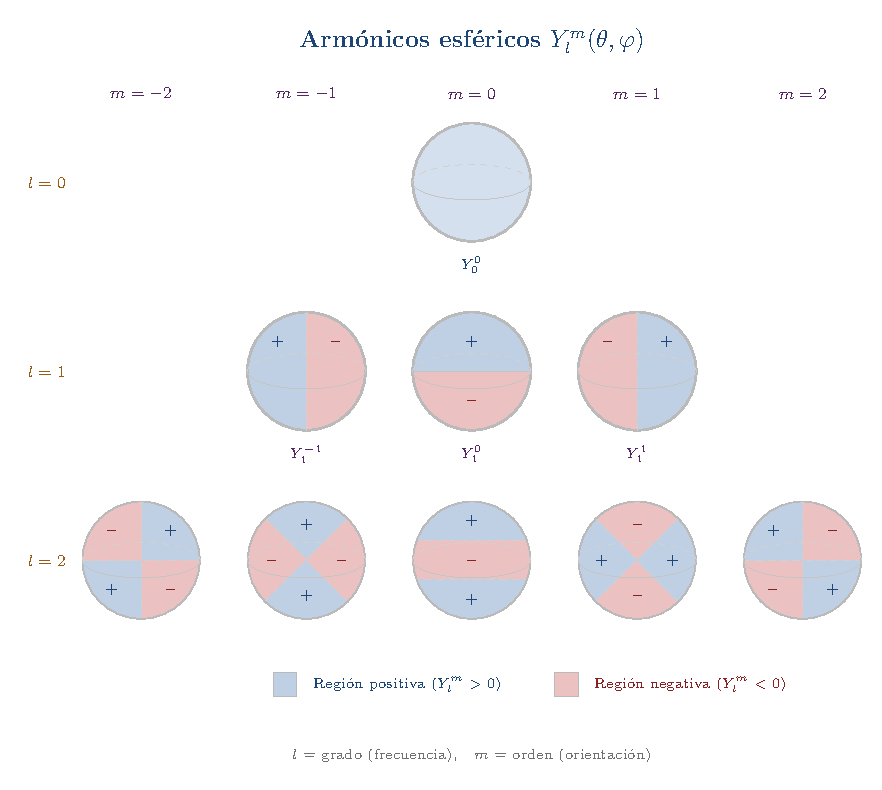
\includegraphics[width=0.80\textwidth]{images/spherical_harmonics}
	\caption[Spherical harmonics $Y_l^m$]{Spherical harmonics $Y_l^m(\theta, \varphi)$ for degrees $l = 0, 1, 2$. The degree $l$ controls the frequency (number of oscillations) and the order $m$ determines the orientation. Blue and red regions represent positive and negative values respectively.}
	\label{fig:spherical_harmonics}
\end{figure}

\subsubsection{The Rotation Group SO(3)}

The special orthogonal group SO(3) consists of all rotations in three-dimensional space that preserve the origin:

\begin{definition}[Group SO(3)]
$SO(3) = \{R \in \mathbb{R}^{3 \times 3} : R^T R = I, \det(R) = 1\}$

Each element can be parameterized by Euler angles $(\alpha, \beta, \gamma)$ or by the rotation axis $\mathbf{n} \in S^2$ and angle $\theta \in [0, 2\pi)$.
\end{definition}

\begin{proposition}[Properties of SO(3)]
The group SO(3) is:
\begin{enumerate}
    \item \textbf{Non-abelian}: In general, $R_1 R_2 \neq R_2 R_1$
    \item \textbf{Compact}: Topologically equivalent to $\mathbb{R}P^3$ (real projective space)
    \item \textbf{Three-parameter}: Requires three independent parameters to completely specify a rotation
\end{enumerate}
\end{proposition}

\begin{proof}
(1) \textit{Non-abelian}: It suffices to exhibit a counterexample. Let $R_x$ be the $90°$ rotation about the $x$ axis and $R_z$ the $90°$ rotation about the $z$ axis. Then $R_x R_z (1,0,0)^T = R_x(0,1,0)^T = (0,0,1)^T$ but $R_z R_x (1,0,0)^T = R_z(1,0,0)^T = (0,1,0)^T$, hence $R_x R_z \neq R_z R_x$.

(2) \textit{Compact}: $SO(3) = \{R \in \mathbb{R}^{3\times 3} : R^TR = I, \det R = 1\}$ is closed in $\mathbb{R}^{9}$ (preimage of regular values under continuous functions) and bounded ($\|R\|_F^2 = \operatorname{tr}(R^TR) = 3$ for all $R \in SO(3)$), hence compact by Heine-Borel. Topological equivalence with $\mathbb{R}P^3$ is established via the axis-angle parameterization: each rotation is identified with a vector $\theta \mathbf{n}$ with $\|\mathbf{n}\| = 1$ and $\theta \in [0, \pi]$, where $(\pi, \mathbf{n})$ and $(\pi, -\mathbf{n})$ represent the same rotation.

(3) \textit{Three-parameter}: $SO(3) \subset \mathbb{R}^{3 \times 3}$ has 9 entries. The conditions $R^TR = I$ impose 6 independent equations (the matrix $R^TR - I$ is symmetric, with 6 independent entries), and $\det R = 1$ is redundant (it follows from $R^TR = I$ and connectedness). Thus, $\dim(SO(3)) = 9 - 6 = 3$.
\end{proof}

This non-commutative structure introduces significant complexities compared to SO(2), requiring more sophisticated tools from harmonic analysis.

\subsubsection{Spherical Harmonic Analysis}

Harmonic analysis on the sphere $S^2$ provides the theoretical basis for constructing SO(3)-equivariant convolutions.

\paragraph{Spherical Harmonics}

\begin{definition}[Spherical Harmonics]
The spherical harmonics $Y_l^m(\theta, \phi)$ form a complete orthonormal basis for $L^2(S^2)$:
\begin{equation}
Y_l^m(\theta, \phi) = \sqrt{\frac{2l+1}{4\pi}\frac{(l-|m|)!}{(l+|m|)!}} P_l^{|m|}(\cos \theta) e^{im\phi}
\end{equation}
where $P_l^m$ are the associated Legendre polynomials, $l \geq 0$ is the degree and $|m| \leq l$ is the order.
\end{definition}

\begin{theorem}[Spherical Harmonic Expansion]
Every function $f \in L^2(S^2)$ admits the expansion:
\begin{equation}
f(\theta, \phi) = \sum_{l=0}^{\infty} \sum_{m=-l}^{l} f_l^m Y_l^m(\theta, \phi)
\end{equation}
with coefficients $f_l^m = \int_{S^2} f(\mathbf{x}) \overline{Y_l^m(\mathbf{x})} d\mathbf{x}$.

See Section~\ref{sec:expansion_armonicos_esfericos} of \autoref{ch:teoremas_complementarios} for the proof of completeness.
\end{theorem}

\paragraph{Transformation under Rotations}

The fundamental property that makes spherical harmonics useful is their behavior under rotations:

\begin{theorem}[Transformation of Spherical Harmonics]
Under a rotation $R \in SO(3)$, spherical harmonics transform as:
\begin{equation}
Y_l^m(R^{-1}\mathbf{x}) = \sum_{m'=-l}^{l} D_{m'm}^{(l)}(R) Y_l^{m'}(\mathbf{x})
\end{equation}
where $D^{(l)}(R)$ is the irreducible representation matrix of dimension $(2l+1) \times (2l+1)$ of SO(3).
\end{theorem}

\begin{proof}
The spherical harmonics $\{Y_l^m\}_{m=-l}^{l}$ form a basis of the subspace $\mathcal{H}_l$ of homogeneous harmonic polynomials of degree $l$ restricted to $S^2$. This subspace is invariant under the action of $SO(3)$: if $R \in SO(3)$ and $Y_l^m \in \mathcal{H}_l$, then $Y_l^m \circ R^{-1} \in \mathcal{H}_l$ (since composition with a rotation preserves both homogeneity and harmonicity, because $\Delta$ commutes with rotations). Since $\mathcal{H}_l$ is of dimension $2l+1$ and invariant, the function $Y_l^m(R^{-1}\mathbf{x})$ is expressed as a linear combination of the basis: $Y_l^m(R^{-1}\mathbf{x}) = \sum_{m'} D_{m'm}^{(l)}(R) Y_l^{m'}(\mathbf{x})$, where the coefficients $D_{m'm}^{(l)}(R) = \int_{S^2} Y_l^m(R^{-1}\mathbf{x}) \overline{Y_l^{m'}(\mathbf{x})} \, d\mathbf{x}$ define the representation matrix. The irreducibility of $D^{(l)}$ follows from the fact that $\mathcal{H}_l$ admits no proper invariant subspaces under $SO(3)$.
\end{proof}

This property is the key to constructing equivariant filters: the coefficients of different degrees $l$ mix only among harmonics of the same degree.

\subsubsection{Architecture of Spherical CNNs}

Spherical CNNs, introduced by Cohen et al.~\citep{cohen2018sphericalcnns}, extend the group equivariance framework to the sphere through the direct use of spherical harmonic analysis.

\begin{example}[Construction of an Equivariant Layer on $S^2$]\label{ex:spherical_equivariant_layer_cnn}
Consider the sphere $S^2 = SO(3)/SO(2)$ for three-dimensional directional data. A function $f: S^2 \rightarrow \mathbb{R}^{d'}$ is $SO(3)$-equivariant if $f(R \cdot \mathbf{x}) = \rho(R) f(\mathbf{x})$ for every rotation $R \in SO(3)$.

To construct a spherical convolutional layer:
\begin{enumerate}
    \item \textbf{Representation}: We choose the representation $\rho_\ell: SO(3) \rightarrow GL(\mathbb{R}^{d_\ell})$ for layer $\ell$
    \item \textbf{Spherical kernel}: The kernel $\psi: S^2 \rightarrow \mathbb{R}^{d_{\ell+1} \times d_\ell}$ must satisfy:
    \begin{equation}
    \psi(R \cdot \omega) = \rho_{\ell+1}(R) \psi(\omega) \rho_\ell(R)^{-1}
    \end{equation}
    \item \textbf{Spherical convolution}: The output is computed as:
    \begin{equation}
    (f * \psi)(\mathbf{x}) = \int_{S^2} f(\omega) \psi(R_{\mathbf{x} \leftarrow \omega}) \, d\omega
    \end{equation}
\end{enumerate}

This construction underpins Spherical \glspl{CNN}, where the spherical harmonics $Y_\ell^m$ provide the irreducible representations of $SO(3)$.
\end{example}

\paragraph{Representation of Spherical Signals}

Instead of operating on pixels in a rectangular grid, Spherical CNNs directly process functions defined on $S^2$:

\begin{definition}[Spherical Signal]
A spherical signal with $C$ channels is a function $f: S^2 \to \mathbb{R}^C$ that can be represented as:
\begin{equation}
f(\mathbf{x}) = \sum_{l=0}^{L} \sum_{m=-l}^{l} \mathbf{f}_l^m Y_l^m(\mathbf{x})
\end{equation}
where $\mathbf{f}_l^m \in \mathbb{R}^C$ are per-channel coefficient vectors.
\end{definition}

\paragraph{Equivariant Spherical Convolution}

Convolution on the sphere is defined using the group structure of SO(3):

\begin{definition}[SO(3) Convolution]
For functions $f: SO(3) \to \mathbb{R}^{C_{\text{in}}}$ and kernel $\psi: SO(3) \to \mathbb{R}^{C_{\text{out}} \times C_{\text{in}}}$:
\begin{equation}
(f \star \psi)(g) = \int_{SO(3)} f(h) \psi(g^{-1}h) dh
\end{equation}
where $dh$ is the Haar measure on SO(3).
\end{definition}

\begin{theorem}[Equivariance of Spherical Convolution]
The SO(3) convolution is equivariant: if $g \cdot f(x) = f(g^{-1}x)$, then:
\begin{equation}
g \cdot (f \star \psi) = (g \cdot f) \star \psi
\end{equation}
\end{theorem}

\begin{proof}
Let $g \in SO(3)$. We compute $(g \cdot f) \star \psi$ using the definition of convolution:
\begin{align}
[(g \cdot f) \star \psi](x) &= \int_{SO(3)} (g \cdot f)(h) \, \psi(x^{-1}h) \, dh = \int_{SO(3)} f(g^{-1}h) \, \psi(x^{-1}h) \, dh
\end{align}
With the change of variable $h' = g^{-1}h$ (i.e., $h = gh'$) and using the left-invariance of the Haar measure ($dh = dh'$):
\begin{align}
&= \int_{SO(3)} f(h') \, \psi(x^{-1}gh') \, dh' = \int_{SO(3)} f(h') \, \psi((g^{-1}x)^{-1}h') \, dh' = (f \star \psi)(g^{-1}x)
\end{align}
This is exactly $[g \cdot (f \star \psi)](x) = (f \star \psi)(g^{-1}x)$, which proves equivariance.
\end{proof}

\subsubsection{Implementation via Spherical FFT}

The efficient implementation of Spherical CNNs requires the use of spherical fast Fourier transforms (S-FFT) to accelerate convolutions in the frequency domain.

\paragraph{Spherical Fourier Transform}

\begin{definition}[Forward S-FFT]
The forward transform computes the spherical harmonic coefficients:
\begin{equation}
\hat{f}_l^m = \int_{S^2} f(\theta, \phi) \overline{Y_l^m(\theta, \phi)} \sin \theta \, d\theta \, d\phi
\end{equation}
\end{definition}

\begin{definition}[Inverse S-FFT]
The inverse transform reconstructs the spatial function:
\begin{equation}
f(\theta, \phi) = \sum_{l=0}^{L} \sum_{m=-l}^{l} \hat{f}_l^m Y_l^m(\theta, \phi)
\end{equation}
\end{definition}

\paragraph{Convolution in the Spectral Domain}

The convolution theorem extends naturally to the spherical case:

\begin{theorem}[Spherical Convolution Theorem]
In the spectral domain, convolution reduces to pointwise multiplication within each degree-$l$ subspace:
\begin{equation}
\widehat{(f \star \psi)}_l^m = \sum_{m'=-l}^{l} \hat{f}_l^{m'} \hat{\psi}_l^{m'm}
\end{equation}
where $\hat{\psi}_l^{m'm}$ are the spectral components of the kernel.
\end{theorem}

\begin{proof}
We expand $f$ and $\psi$ in spherical harmonics. The convolution $(f \star \psi)(g) = \int_{SO(3)} f(h) \psi(g^{-1}h) \, dh$ is expressed in the spectral domain using the Fourier transform over $SO(3)$: $\hat{F}^{(l)}_{mm'} = \int_{SO(3)} F(g) D^{(l)}_{mm'}(g) \, dg$. By the convolution theorem for compact groups, the transform of the convolution is the matrix product of the transforms:
\[
\widehat{(f \star \psi)}^{(l)} = \hat{f}^{(l)} \cdot \hat{\psi}^{(l)}
\]
where the product is matrix multiplication in the indices $m, m'$ within each degree-$l$ block. Componentwise, this gives $\widehat{(f \star \psi)}_l^m = \sum_{m'=-l}^{l} \hat{f}_l^{m'} \hat{\psi}_l^{m'm}$.
\end{proof}

\begin{algorithm}[h]
\caption{Efficient Spherical CNN Convolution}
\label{alg:spherical_conv}
\begin{algorithmic}[1]
\Require Spherical signal $f$, spectral kernel $\hat{\psi}$, maximum degree $L$
\Ensure Convolved signal in the spectral domain
\State Compute S-FFT: $\hat{f}_l^m = \text{S-FFT}(f)$
\For{$l = 0$ to $L$}
    \For{$m = -l$ to $l$}
        \State $\hat{g}_l^m = \sum_{m'} \hat{f}_l^{m'} \hat{\psi}_l^{m'm}$
    \EndFor
\EndFor
\State \textbf{return} $\{\hat{g}_l^m\}$ (keep spectral representation for subsequent layers)
\end{algorithmic}
\end{algorithm}

\subsubsection{Extension to 3D Volumetric Data}

Spherical CNNs extend naturally to three-dimensional volumetric data by combining spherical harmonic analysis with radial processing.

\paragraph{3D Spherical Coordinates}

For volumetric data $f: \mathbb{R}^3 \to \mathbb{R}$, the decomposition in spherical coordinates $(r, \theta, \phi)$ is used:

\begin{equation}
f(r, \theta, \phi) = \sum_{l=0}^{L} \sum_{m=-l}^{l} f_l^m(r) Y_l^m(\theta, \phi)
\end{equation}

where $f_l^m(r)$ are radial functions that capture the variation with respect to the distance from the origin.

\paragraph{3D Steerable CNNs}

The complete formulation for 3D data, developed by Weiler et al.~\citep{weiler2018steerable}, combines:

\begin{enumerate}
    \item \textbf{Radial processing}: 1D convolutions along radial rays
    \item \textbf{Angular mixing}: Linear transformations between spherical harmonic coefficients
    \item \textbf{SO(3) equivariance}: Preservation of the irreducible representation structure
\end{enumerate}

\begin{definition}[3D Steerable Kernel]
A 3D steerable kernel is parameterized as:
\begin{equation}
K(r, \theta, \phi) = \sum_{l=0}^{L} \sum_{i=1}^{I} R_i(r) \sum_{m=-l}^{l} W_{l,i}^m Y_l^m(\theta, \phi)
\end{equation}
where $R_i(r)$ are radial basis functions and $W_{l,i}^m$ are learnable parameters.
\end{definition}

\subsubsection{Applications in Spherical Domains}

\paragraph{Analysis of Omnidirectional Images}

Spherical CNNs have demonstrated significant advantages in the processing of $360^\circ$ images:

\begin{itemize}
    \item \textbf{Object recognition}: Robust detection independent of camera orientation
    \item \textbf{Virtual reality}: Efficient processing of immersive content
    \item \textbf{Robotics}: Navigation based on omnidirectional vision
\end{itemize}

\paragraph{Climate and Geophysical Modeling}

In Earth sciences, Spherical CNNs provide natural tools for:

\begin{itemize}
    \item \textbf{Weather prediction}: Models that respect the spherical geometry of the planet
    \item \textbf{Ocean current analysis}: Processing of vector data on the sphere
    \item \textbf{Satellite monitoring}: Analysis of Earth observation data
\end{itemize}

\paragraph{Computational Astrophysics}

The natural spherical structure of astronomical data makes Spherical CNNs particularly appropriate:

\begin{example}[Cosmic Microwave Background]
The analysis of anisotropies in the cosmic microwave background (CMB) requires processing of signals defined over the complete celestial sphere. Spherical CNNs can detect cosmological patterns while preserving all rotational symmetries.
\end{example}

\subsubsection{Performance Comparison}

Comparative experiments demonstrate the advantages of Spherical CNNs over conventional methods:

\begin{table}[h]
\centering
\begin{tabular}{|l|c|c|c|}
\hline
\textbf{Method} & \textbf{Omnidirectional MNIST} & \textbf{Climate Pattern} & \textbf{Spherical CIFAR} \\
\hline
CNN + Equirectangular & 89.2\% & 76.4\% & 72.8\% \\
CNN + Cubemap & 91.7\% & 79.1\% & 76.2\% \\
Spherical CNN & \textbf{96.4\%} & \textbf{87.3\%} & \textbf{83.1\%} \\
\hline
\end{tabular}
\caption{Accuracy on synthetic and real spherical datasets}
\label{tab:spherical_performance}
\end{table}

\paragraph{Computational Efficiency}

The complexity of Spherical CNNs depends on the maximum degree $L$ of the spherical harmonics:

\begin{itemize}
    \item \textbf{Space complexity}: $O(L^2)$ coefficients per spherical location
    \item \textbf{Time complexity}: $O(L^3)$ for S-FFT, $O(L^2)$ for spectral convolutions
    \item \textbf{Parallelization}: Spectral transforms parallelize efficiently
\end{itemize}

\subsubsection{Extensions and Recent Developments}

\paragraph{Spherical CNNs on Unstructured Grids}

Recent developments have extended Spherical CNNs to non-uniform grids~\citep{cohen2021spherical}:

\begin{itemize}
    \item \textbf{Adaptive meshes}: Support for variable resolutions depending on the region
    \item \textbf{Icosahedral grids}: Spherical discretizations with improved symmetry properties
    \item \textbf{Spectral interpolation}: Techniques for handling irregular samplings
\end{itemize}

\paragraph{Hybrid Architectures}

Current research explores combinations with other approaches:

\begin{enumerate}
    \item \textbf{Gauge Equivariant Networks}: Combination with local gauge symmetries~\citep{cohen2019gaugeequivariantconvolutional}
    \item \textbf{Spherical transformers}: Integration of attention mechanisms with SO(3) equivariance
    \item \textbf{Graph Neural Networks}: Treatment of spherical data as graphs on the sphere
\end{enumerate}

\subsubsection{Limitations and Challenges}

\paragraph{Computational Challenges}

\begin{enumerate}
    \item \textbf{Spectral complexity}: The $O(L^3)$ cost of S-FFTs limits the angular resolution
    \item \textbf{Numerical precision}: High-degree spherical harmonics are sensitive to floating-point errors
    \item \textbf{Memory}: Storing spectral coefficients can be prohibitive for large $L$
\end{enumerate}

\paragraph{Theoretical Limitations}

\begin{itemize}
    \item \textbf{Bandlimit assumption}: Real data may not be spectrally band-limited
    \item \textbf{Sampling artifacts}: Discretizations introduce spectral aliasing
    \item \textbf{Boundary effects}: Handling partial regions of the sphere requires specialized techniques
\end{itemize}

\subsubsection{Unifying Perspective}

Spherical CNNs represent a natural and powerful extension of the group equivariance framework from SO(2) toward SO(3), demonstrating how the principles of harmonic analysis can be integrated directly into deep learning architectures. Their success illustrates a fundamental principle: the alignment between the intrinsic symmetries of the data and the architectural inductive biases produces significant improvements in both efficiency and performance.

The progression from standard \glspl{CNN} → discrete \glspl{GCNN} → SO(2) Steerable \glspl{CNN} → SO(3) Spherical \glspl{CNN} illustrates an evolution toward increasingly geometrically aware architectures. This trend continues toward even more general formulations, including networks equivariant to arbitrary Lie groups and convolutions over general Riemannian manifolds.

The theoretical framework developed for Spherical CNNs provides the conceptual tools needed to address data with even more complex geometries, establishing the foundations for the development of Geometric Deep Learning in arbitrary non-Euclidean domains.

\subsection{Non-Compact Groups (E(3), SE(3))}\label{subsec:grupos_no_compactos}

The Euclidean groups $E(n)$ and rigid-motion groups $SE(3)$ represent fundamental extensions toward non-compact groups that incorporate translations together with rotations. These architectures are especially relevant for the processing of 3D point clouds, molecular systems, and particle analysis, where the symmetries include both rotations and translations in three-dimensional space.

The transition from compact groups such as $SO(2)$ and $SO(3)$ toward non-compact groups introduces significant mathematical and computational challenges. While compact groups admit finite Haar measures that allow direct integration over the group, non-compact groups require more sophisticated techniques to construct efficient equivariant representations.

\subsubsection{Mathematical Structure of Non-Compact Groups}

\paragraph{The Euclidean Group E(n)}

The \textit{Euclidean group} $E(n) = \mathbb{R}^n \rtimes O(n)$ is the group of all isometries of $\mathbb{R}^n$ (\autoref{def:grupo_e_n} of \autoref{ch:gdl}).\label{def:grupo_euclidiano}

Each element $g \in E(n)$ is represented as a pair $(R, \mathbf{t})$ with $R \in O(n)$ and $\mathbf{t} \in \mathbb{R}^n$, acting on $\mathbf{x} \in \mathbb{R}^n$ via:
\begin{equation}
g \cdot \mathbf{x} = R\mathbf{x} + \mathbf{t}
\end{equation}

The group operation is defined as:
\begin{equation}
(R_1, \mathbf{t}_1) \circ (R_2, \mathbf{t}_2) = (R_1 R_2, R_1 \mathbf{t}_2 + \mathbf{t}_1)
\end{equation}

\begin{proposition}[Properties of $E(n)$]
The Euclidean group $E(n)$ satisfies:
\begin{enumerate}
    \item \textbf{Non-compact}: The subgroup of translations $\mathbb{R}^n$ is non-compact
    \item \textbf{Lie group}: Differentiable manifold of dimension $n + \frac{n(n-1)}{2}$
    \item \textbf{Semidirect product}: $\mathbb{R}^n$ is a normal subgroup
\end{enumerate}
\end{proposition}

\begin{proof}
(1) \textit{Non-compact}: The subgroup of pure translations $\{(I, \mathbf{t}) : \mathbf{t} \in \mathbb{R}^n\} \cong \mathbb{R}^n$ is unbounded, hence $E(n)$ is not compact.

(2) \textit{Lie group}: $E(n)$ is realized as a closed subgroup of $GL(n+1, \mathbb{R})$ via the matrix representation $(R, \mathbf{t}) \mapsto \begin{psmallmatrix} R & \mathbf{t} \\ 0 & 1 \end{psmallmatrix}$. The dimension is $n$ (translations) $+ \frac{n(n-1)}{2}$ (dimension of $O(n)$, by the count $n^2 - \frac{n(n+1)}{2}$ constraints from orthogonality $R^TR = I$).

(3) \textit{Semidirect product}: For $(R_1, \mathbf{t}_1), (R_2, \mathbf{t}_2) \in E(n)$, conjugation of a pure translation $(I, \mathbf{t})$ gives $(R, \mathbf{s})(I, \mathbf{t})(R, \mathbf{s})^{-1} = (I, R\mathbf{t})$, which remains a pure translation. Thus, the translations form a normal subgroup, and the group law $(R_1, \mathbf{t}_1) \cdot (R_2, \mathbf{t}_2) = (R_1 R_2, R_1 \mathbf{t}_2 + \mathbf{t}_1)$ is exactly that of the semidirect product $\mathbb{R}^n \rtimes O(n)$.
\end{proof}

\paragraph{The Group of Rigid Motions SE(n)}

The \textit{special Euclidean group} $SE(n) = \mathbb{R}^n \rtimes SO(n)$ is the subgroup of $E(n)$ that preserves orientation (\autoref{def:grupo_se_n} of \autoref{ch:gdl}).\label{def:grupo_se_n_cnn}

For $n = 3$, the group $SE(3)$ is fundamental in robotics, computer vision and computational chemistry, since it captures all rigid transformations that preserve distances and orientation in three-dimensional space.

\paragraph{Representations of Non-Compact Groups}

Unlike compact groups, where all unitary irreducible representations are finite-dimensional, non-compact groups admit infinite-dimensional irreducible representations. However, for practical applications in deep learning, we restrict ourselves to finite-dimensional representations that capture the rotational components.

\begin{proposition}[Decomposition of Representations]\label{prop:descomp_repr_en}
Let $E(n) = \mathbb{R}^n \rtimes O(n)$ be the Euclidean group (semidirect product). In every finite-dimensional representation of $E(n)$ where the translations act trivially, the representation factors through the quotient $E(n)/\mathbb{R}^n \cong O(n)$:
\begin{equation}
\rho(R, \mathbf{t}) = \rho_{O(n)}(R)
\end{equation}
where $\rho_{O(n)}$ is a representation of $O(n)$. Analogously, for $SE(n) = \mathbb{R}^n \rtimes SO(n)$, the representation factors through $SO(n)$. See \citep{DBLP:journals/corr/abs-2104-13478} for a discussion in the context of GDL.
\end{proposition}

\begin{proof}
Let $\rho: E(n) \to GL(V)$ be a finite-dimensional representation where the translations act trivially: $\rho(I, \mathbf{t}) = \operatorname{Id}_V$ for all $\mathbf{t} \in \mathbb{R}^n$. For $(R, \mathbf{t}) \in E(n)$, since $(R, \mathbf{t}) = (R, \mathbf{0}) \cdot (I, R^{-1}\mathbf{t})$, we have $\rho(R, \mathbf{t}) = \rho(R, \mathbf{0}) \cdot \rho(I, R^{-1}\mathbf{t}) = \rho(R, \mathbf{0})$. Defining $\rho_{O(n)}(R) := \rho(R, \mathbf{0})$, one verifies that $\rho_{O(n)}$ is a group homomorphism: $\rho_{O(n)}(R_1 R_2) = \rho(R_1 R_2, \mathbf{0}) = \rho(R_1, \mathbf{0}) \rho(R_2, \mathbf{0}) = \rho_{O(n)}(R_1) \rho_{O(n)}(R_2)$. This proves the factorization $\rho = \rho_{O(n)} \circ \pi$, where $\pi: E(n) \to E(n)/\mathbb{R}^n \cong O(n)$ is the canonical projection.
\end{proof}

This factorization motivates the design of architectures that explicitly separate invariant information (scalar features) from equivariant information (vector coordinates).

\subsubsection{E(n) Equivariant Graph Neural Networks}

The E(n) Equivariant Graph Neural Networks of Satorras et al.~\citep{satorras2021enequivariant} introduce a general framework for Euclidean group equivariance via an architecture that explicitly processes both invariant features and equivariant coordinates.

\paragraph{Foundations of the EGNN Design}

The central idea is to construct messages that depend only on quantities invariant under $E(n)$, while coordinate updates are performed via vector differences that preserve equivariance.

\paragraph{EGNN Architecture}

EGNNs maintain equivariance through the explicit separation of scalar information and vector information. In each layer, the following are processed simultaneously:
\begin{itemize}
    \item \textbf{Scalar features} $h_i \in \mathbb{R}^d$ (invariant under $E(n)$)
    \item \textbf{Coordinates} $\mathbf{x}_i \in \mathbb{R}^n$ (equivariant under $E(n)$)
\end{itemize}

The update in an EGNN layer proceeds in three stages:

\textbf{Stage 1: Construction of invariant messages}

Messages between nodes are constructed using only $E(n)$-invariant quantities:
\begin{equation}\label{eq:egnn_message}
\mathbf{m}_{ij} = \phi_e(h_i, h_j, \|\mathbf{x}_i - \mathbf{x}_j\|^2, a_{ij})
\end{equation}

where:
\begin{itemize}
    \item $h_i, h_j \in \mathbb{R}^d$ are scalar features (inherently invariant)
    \item $\|\mathbf{x}_i - \mathbf{x}_j\|^2$ is the squared Euclidean distance (invariant under isometries)
    \item $a_{ij}$ are optional edge attributes
    \item $\phi_e: \mathbb{R}^{2d+2} \to \mathbb{R}^{d'}$ is an MLP
\end{itemize}

\textbf{Invariance of Distances.} The squared distance is invariant under $E(n)$: for any $(R, \mathbf{t}) \in E(n)$,
\begin{equation}
\|(R\mathbf{x}_i + \mathbf{t}) - (R\mathbf{x}_j + \mathbf{t})\|^2 = \|R(\mathbf{x}_i - \mathbf{x}_j)\|^2 = \|\mathbf{x}_i - \mathbf{x}_j\|^2
\end{equation}
since $R$ is orthogonal and the translations cancel.

\textbf{Stage 2: Equivariant coordinate update}

The coordinates are updated using weighted vector differences:
\begin{equation}\label{eq:egnn_coord_update}
\mathbf{x}_i' = \mathbf{x}_i + C \sum_{j \in \mathcal{N}(i)} (\mathbf{x}_i - \mathbf{x}_j) \phi_x(\mathbf{m}_{ij})
\end{equation}

where:
\begin{itemize}
    \item $\phi_x: \mathbb{R}^{d'} \to \mathbb{R}$ is an MLP that produces scalar coefficients
    \item $C$ is a normalization constant (typically $C = 1/|\mathcal{N}(i)|$)
    \item $\mathcal{N}(i)$ is the neighborhood of node $i$
\end{itemize}

\begin{proposition}[Equivariance of the Coordinate Update]\label{prop:egnn_coord_equivariance}
The update~\eqref{eq:egnn_coord_update} is equivariant under $E(n)$. If we apply $(R, \mathbf{t}) \in E(n)$ to all coordinates, then:
\begin{equation}
\mathbf{x}_i'^{(g)} = R\mathbf{x}_i' + \mathbf{t}
\end{equation}
where $\mathbf{x}_i'^{(g)}$ denotes the updated coordinate after transforming the inputs.
\end{proposition}

\begin{proof}
Consider the transformed coordinates $\tilde{\mathbf{x}}_i = R\mathbf{x}_i + \mathbf{t}$. The messages $\mathbf{m}_{ij}$ are invariant under this transformation (by construction using distances). The update of the transformed coordinates is:
\begin{align}
\tilde{\mathbf{x}}_i' &= \tilde{\mathbf{x}}_i + C \sum_{j \in \mathcal{N}(i)} (\tilde{\mathbf{x}}_i - \tilde{\mathbf{x}}_j) \phi_x(\mathbf{m}_{ij}) \\
&= R\mathbf{x}_i + \mathbf{t} + C \sum_{j \in \mathcal{N}(i)} ((R\mathbf{x}_i + \mathbf{t}) - (R\mathbf{x}_j + \mathbf{t})) \phi_x(\mathbf{m}_{ij}) \\
&= R\mathbf{x}_i + \mathbf{t} + C \sum_{j \in \mathcal{N}(i)} R(\mathbf{x}_i - \mathbf{x}_j) \phi_x(\mathbf{m}_{ij}) \\
&= R\left(\mathbf{x}_i + C \sum_{j \in \mathcal{N}(i)} (\mathbf{x}_i - \mathbf{x}_j) \phi_x(\mathbf{m}_{ij})\right) + \mathbf{t} \\
&= R\mathbf{x}_i' + \mathbf{t}
\end{align}
demonstrating equivariance.
\end{proof}

\textbf{Stage 3: Invariant feature update}

The scalar features are updated using aggregated messages:
\begin{align}
\mathbf{m}_i &= \sum_{j \in \mathcal{N}(i)} \mathbf{m}_{ij} \label{eq:egnn_aggregate}\\
h_i' &= \phi_h(h_i, \mathbf{m}_i) \label{eq:egnn_feature_update}
\end{align}

where $\phi_h: \mathbb{R}^{d + d'} \to \mathbb{R}^d$ is an MLP. This update is trivially $E(n)$-invariant since it operates only on invariant scalar quantities.

\paragraph{Equivariance Properties}

The architecture guarantees that for any Euclidean transformation $g = (R, \mathbf{t}) \in E(n)$:
\begin{align}
h_i'(g \cdot \mathbf{X}) &= h_i'(\mathbf{X}) \quad \text{(invariance)} \\
\mathbf{x}_i'(g \cdot \mathbf{X}) &= g \cdot \mathbf{x}_i'(\mathbf{X}) \quad \text{(equivariance)}
\end{align}

where $g \cdot \mathbf{X} = \{R\mathbf{x}_i + \mathbf{t}\}_{i=1}^N$ denotes the transformation of all coordinates.

\begin{example}[EGNN Message Passing for a Molecular System]\label{ex:egnn_molecular}
Consider a small molecule with three atoms located at:
\begin{equation}
\mathbf{x}_1 = \begin{pmatrix} 0 \\ 0 \\ 0 \end{pmatrix}, \quad
\mathbf{x}_2 = \begin{pmatrix} 1.5 \\ 0 \\ 0 \end{pmatrix}, \quad
\mathbf{x}_3 = \begin{pmatrix} 0.75 \\ 1.3 \\ 0 \end{pmatrix}
\end{equation}

With initial scalar features $h_1 = [6.0]$ (carbon), $h_2 = [1.0]$ (hydrogen), $h_3 = [8.0]$ (oxygen).

\textbf{Step 1: Distance computation}
\begin{align}
d_{12}^2 &= \|\mathbf{x}_1 - \mathbf{x}_2\|^2 = 2.25 \\
d_{13}^2 &= \|\mathbf{x}_1 - \mathbf{x}_3\|^2 = 0.75^2 + 1.3^2 = 2.2525 \\
d_{23}^2 &= \|\mathbf{x}_2 - \mathbf{x}_3\|^2 = 0.75^2 + 1.3^2 = 2.2525
\end{align}

\textbf{Step 2: Messages} (using a simplified $\phi_e$)
\begin{equation}
\mathbf{m}_{12} = \phi_e(h_1, h_2, d_{12}^2) = \text{MLP}([6.0, 1.0, 2.25])
\end{equation}

\textbf{Step 3: Coordinate update}
\begin{equation}
\mathbf{x}_1' = \mathbf{x}_1 + \frac{1}{2}\left[(\mathbf{x}_1 - \mathbf{x}_2)\phi_x(\mathbf{m}_{12}) + (\mathbf{x}_1 - \mathbf{x}_3)\phi_x(\mathbf{m}_{13})\right]
\end{equation}

This update automatically preserves equivariance: if we rotate the entire molecule, the updated coordinates rotate in the same way.
\end{example}

\subsubsection{SE(3)-Transformers}

Fuchs et al.~\citep{fuchs2020se3transformers} develop the SE(3)-Transformers, which combine equivariance to the group of rigid motions $SE(3)$ with attention mechanisms, providing a more expressive architecture than EGNNs by using complete tensor representations of $SO(3)$.

\paragraph{The SE(3) Group and its Properties}

\begin{definition}[Group SE(3)]
The group of rigid motions $SE(3) = \mathbb{R}^3 \rtimes SO(3)$ consists of all transformations that preserve distances and orientation in $\mathbb{R}^3$.
\end{definition}

Each element of $SE(3)$ is written as $(R, \mathbf{t})$ where $R \in SO(3)$ and $\mathbf{t} \in \mathbb{R}^3$, acting on points via:
\begin{equation}
(R, \mathbf{t}) \cdot \mathbf{x} = R\mathbf{x} + \mathbf{t}
\end{equation}

\begin{proposition}[Differences with E(3)]
$SE(3) \subset E(3)$ is the subgroup that preserves orientation (it does not include reflections). This restriction is crucial in applications where chirality matters, such as in molecular chemistry.
\end{proposition}

\begin{proof}
$SE(3) = \mathbb{R}^3 \rtimes SO(3)$ consists of pairs $(R, \mathbf{t})$ with $R \in SO(3)$ (i.e., $\det R = +1$), while $E(3) = \mathbb{R}^3 \rtimes O(3)$ also includes elements with $\det R = -1$ (reflections). The inclusion $SE(3) \subset E(3)$ is strict: for example, the reflection $(x,y,z) \mapsto (-x,y,z)$ belongs to $E(3)$ but not to $SE(3)$. In molecular chemistry, a molecule and its mirror image (enantiomer) may have different properties (chirality), so it is necessary to distinguish between transformations that preserve ($SE(3)$) and those that invert ($O(3) \setminus SO(3)$) orientation.
\end{proof}

\paragraph{Irreducible Representations of SO(3)}

Unlike EGNNs, which use only scalar features and position vectors, SE(3)-Transformers work with complete tensor representations of $SO(3)$.

\begin{definition}[Irreducible Representations of SO(3)]\label{def:irreps_so3}
The irreducible representations of $SO(3)$ are classified by non-negative integers $l = 0, 1, 2, \ldots$ (degree or angular momentum). The degree-$l$ representation has dimension $2l + 1$ and is denoted $\rho^{(l)}: SO(3) \to \mathbb{R}^{(2l+1) \times (2l+1)}$.

For a rotation $R \in SO(3)$ parameterized by Euler angles $(\alpha, \beta, \gamma)$, the matrix elements are:
\begin{equation}
D_{mm'}^{(l)}(\alpha, \beta, \gamma) = e^{-im\alpha} d_{mm'}^{(l)}(\beta) e^{-im'\gamma}
\end{equation}
where $d_{mm'}^{(l)}$ are the Wigner small functions.
\end{definition}

\begin{example}[Low Degrees of SO(3)]
\leavevmode
\begin{itemize}
    \item $l = 0$: Scalars (dimension 1), invariant under rotations
    \item $l = 1$: Vectors (dimension 3), transform as $\mathbf{v}' = R\mathbf{v}$
    \item $l = 2$: Symmetric traceless second-order tensors (dimension 5)
\end{itemize}
\end{example}

\paragraph{Feature Tensors}

SE(3)-Transformers use tensor representations that transform according to irreducible representations of $SO(3)$:

\begin{definition}[Feature Tensor]\label{def:feature_tensor_se3}
A \textit{feature tensor} of type $l$ at node $i$ is a vector $\mathbf{f}_i^{(l)} \in \mathbb{R}^{2l+1}$ that transforms under rotations $R \in SO(3)$ as:
\begin{equation}
(\mathbf{f}_i^{(l)})' = D^{(l)}(R) \mathbf{f}_i^{(l)}
\end{equation}
where $D^{(l)}(R)$ is the degree-$l$ irreducible representation matrix.
\end{definition}

In practice, each node maintains multiple copies (multiplicities) of each irreducible type:
\begin{equation}
\mathbf{F}_i = \bigoplus_{l=0}^{L_{\max}} \bigoplus_{k=1}^{n_l} \mathbf{f}_{i,k}^{(l)}
\end{equation}
where $n_l$ is the multiplicity of type $l$ and $L_{\max}$ is the maximum degree.

\paragraph{Tensor Products and Channel Mixing}

The combination of feature tensors of different types requires the use of Clebsch-Gordan tensor products, which guarantee equivariance under $SO(3)$.

\begin{theorem}[Clebsch-Gordan Decomposition]\label{thm:clebsch_gordan}
The tensor product of two irreducible representations of $SO(3)$ decomposes as a direct sum of irreducibles:
\begin{equation}
\rho^{(l_1)} \otimes \rho^{(l_2)} = \bigoplus_{l=|l_1-l_2|}^{l_1+l_2} \rho^{(l)}
\end{equation}

The Clebsch-Gordan coefficients $C_{l_1 m_1, l_2 m_2}^{l m}$ implement this decomposition:
\begin{equation}
(f^{(l_1)} \otimes g^{(l_2)})^{(l)}_m = \sum_{m_1=-l_1}^{l_1} \sum_{m_2=-l_2}^{l_2} C_{l_1 m_1, l_2 m_2}^{l m} f^{(l_1)}_{m_1} g^{(l_2)}_{m_2}
\end{equation}

See Section~\ref{sec:clebsch_gordan} of \autoref{ch:teoremas_complementarios} for the complete proof.
\end{theorem}

\textbf{Selection Rule.} The tensor product produces degrees in the range $|l_1 - l_2| \leq l \leq l_1 + l_2$. For example:
\begin{itemize}
    \item Vector $\times$ Vector ($l=1 \times l=1$): generates $l \in \{0, 1, 2\}$ (scalar + vector + tensor)
    \item Scalar $\times$ Vector ($l=0 \times l=1$): generates only $l=1$ (vector)
\end{itemize}

\paragraph{Equivariant Attention Mechanism}

The key challenge is to design attention weights that are invariant under $SE(3)$, allowing the weighted combination of tensor features to preserve equivariance.

The attention weights are computed using only the scalar component ($l=0$) of the feature tensors:
\begin{equation}\label{eq:se3_attention_weights}
\alpha_{ij} = \text{softmax}_j\left(\text{MLP}\left(\mathbf{f}_i^{(0)} \oplus \mathbf{f}_j^{(0)} \oplus h(r_{ij})\right)\right)
\end{equation}

where:
\begin{itemize}
    \item $\mathbf{f}_i^{(0)}, \mathbf{f}_j^{(0)}$ are the scalar components (invariant)
    \item $r_{ij} = \|\mathbf{x}_i - \mathbf{x}_j\|$ is the distance (invariant under $SE(3)$)
    \item $h(r_{ij})$ is a radial embedding of the distance
    \item $\oplus$ denotes concatenation
\end{itemize}

\begin{proposition}[Invariance of the Attention Weights]
The weights $\alpha_{ij}$ defined in~\eqref{eq:se3_attention_weights} are invariant under $SE(3)$: for any $(R, \mathbf{t}) \in SE(3)$,
\begin{equation}
\alpha_{ij}((R, \mathbf{t}) \cdot \{\mathbf{x}_k\}, \{\mathbf{F}_k\}) = \alpha_{ij}(\{\mathbf{x}_k\}, \{\mathbf{F}_k\})
\end{equation}
\end{proposition}

\begin{proof}
The attention weights depend on the positions $\mathbf{x}_k$ only through the differences $\mathbf{x}_i - \mathbf{x}_j$ and the norms $\|\mathbf{x}_i - \mathbf{x}_j\|$. Under the action $(R, \mathbf{t}) \in SE(3)$: the transformed difference is $R\mathbf{x}_i + \mathbf{t} - (R\mathbf{x}_j + \mathbf{t}) = R(\mathbf{x}_i - \mathbf{x}_j)$, and the norm $\|R(\mathbf{x}_i - \mathbf{x}_j)\| = \|\mathbf{x}_i - \mathbf{x}_j\|$ by the orthogonality of $R$. Since $\alpha_{ij}$ is computed as a function of $\|\mathbf{x}_i - \mathbf{x}_j\|$ and of the invariant features $\mathbf{F}_k$ (which by hypothesis are invariant under $SE(3)$), the attention weights are invariant.
\end{proof}

\paragraph{Equivariant Linear Combination}

Once the invariant attention weights are computed, the update of the tensor features is performed via a weighted linear combination within each irreducible type:

\begin{equation}\label{eq:se3_feature_update}
\mathbf{f}_i^{(l), \text{new}} = \sum_{j \in \mathcal{N}(i)} \alpha_{ij} \cdot W_{ij}^{(l)} \mathbf{f}_j^{(l)}
\end{equation}

where $W_{ij}^{(l)}$ are learnable mixing matrices that act within the type-$l$ subspace.

\begin{theorem}[Equivariance of SE(3)-Transformers]\label{thm:se3_transformer_equivariance}
The update~\eqref{eq:se3_feature_update} with weights~\eqref{eq:se3_attention_weights} is equivariant: if we transform all positions and features by $(R, \mathbf{t}) \in SE(3)$, then
\begin{equation}
(\mathbf{f}_i^{(l), \text{new}})' = D^{(l)}(R) \mathbf{f}_i^{(l), \text{new}}
\end{equation}
\end{theorem}

\begin{proof}
The attention weights $\alpha_{ij}$ are invariant under $SE(3)$ (by the previous Proposition). The key point is that the matrices $W_{ij}^{(l)}$ in equation~\eqref{eq:se3_feature_update} act as scalar mixing coefficients between channels of the same type $l$, that is, they are multiples of the identity in the $(2l+1)$-dimensional representation subspace. In the implementation of \citet{fuchs2020se3transformers}, the value messages are constructed via TFN-type equivariant kernels~\citep{thomas2018tensorfieldnetworks}, which use Clebsch-Gordan coefficients and learnable radial functions. Therefore, each value message $\mathbf{v}_j^{(l)} = W_{ij}^{(l)} \mathbf{f}_j^{(l)}$ transforms as $(\mathbf{v}_j^{(l)})' = D^{(l)}(R) \mathbf{v}_j^{(l)}$. Then:
\begin{align}
(\mathbf{f}_i^{(l), \text{new}})' &= \sum_j \alpha_{ij} \, (\mathbf{v}_j^{(l)})' = \sum_j \alpha_{ij} \, D^{(l)}(R) \mathbf{v}_j^{(l)} \\
&= D^{(l)}(R) \sum_j \alpha_{ij} \, \mathbf{v}_j^{(l)} = D^{(l)}(R) \mathbf{f}_i^{(l), \text{new}}
\end{align}
where in the second step we use the invariance of $\alpha_{ij}$ and the linearity of $D^{(l)}(R)$. Translations do not affect the tensor features (only the positions), completing the equivariance under $SE(3)$.
\end{proof}

\paragraph{Radial Filters and Spatial Dependence}

To incorporate spatial information, radial filters are used that modulate the weights according to distance:

\begin{equation}
W_{ij}^{(l)} = \sum_{k=1}^{K} w_k^{(l)} R_k(r_{ij})
\end{equation}

where $R_k(r)$ are radial basis functions (typically Gaussians or Bessels) and $w_k^{(l)}$ are learnable parameters.

\subsubsection{Tensor Field Networks}

Thomas et al.~\citep{thomas2018tensorfieldnetworks} introduce Tensor Field Networks (TFNs), providing the fundamental theoretical framework for $SE(3)$-equivariant networks via an elegant formulation based on tensor fields and spherical harmonics.

\paragraph{Tensor Fields as Functions over Points}

\begin{definition}[Tensor Field of Order $l$]\label{def:tensor_field}
A \textit{tensor field} of order $l$ associated with a set of points $\{\mathbf{x}_i\}_{i=1}^N$ is a collection of tensors $\{T_i^{(l)}\}_{i=1}^N$ where each $T_i^{(l)} \in \mathbb{R}^{2l+1}$ transforms according to the degree-$l$ irreducible representation of $SO(3)$:
\begin{equation}
(T_i^{(l)})' = D^{(l)}(R) T_i^{(l)} \quad \text{for } R \in SO(3)
\end{equation}
\end{definition}

In TFNs, each point in a 3D point cloud carries multiple tensor fields of different orders, capturing rich geometric information in an equivariant manner.

\paragraph{Convolution of Tensor Fields}

The fundamental operation in TFNs is the convolution between tensor fields, which must preserve equivariance under $SE(3)$.

\begin{definition}[TFN Convolution]\label{def:tfn_convolution}
The convolution between a tensor field $T^{(l_{\text{in}})}$ and a kernel $W^{(l_{\text{out}}, l_{\text{in}})}$ at point $i$ is defined as:
\begin{equation}\label{eq:tfn_conv}
(T * W)_i^{(l_{\text{out}})} = \sum_{j \in \mathcal{N}(i)} \sum_{l_{\text{in}}} K_{ij}^{(l_{\text{out}}, l_{\text{in}})} T_j^{(l_{\text{in}})}
\end{equation}
where $K_{ij}^{(l_{\text{out}}, l_{\text{in}})}$ is an SE(3)-equivariant kernel that depends on the relative position $\mathbf{r}_{ij} = \mathbf{x}_i - \mathbf{x}_j$.
\end{definition}

\paragraph{Radial-Angular Factorization of the Kernel}

The key design of TFNs is to factorize the kernel into radial (learnable) and angular (fixed, given by spherical harmonics) components:

\begin{equation}\label{eq:tfn_kernel_factorization}
K_{ij}^{(l_{\text{out}}, l_{\text{in}})} = \sum_{l_{\text{filter}}} R^{l_{\text{filter}}}_{l_{\text{out}}, l_{\text{in}}}(r_{ij}) \mathcal{Y}^{(l_{\text{filter}})}(\hat{\mathbf{r}}_{ij})
\end{equation}

where:
\begin{itemize}
    \item $r_{ij} = \|\mathbf{r}_{ij}\|$ is the distance (invariant scalar)
    \item $\hat{\mathbf{r}}_{ij} = \mathbf{r}_{ij} / r_{ij}$ is the unit direction
    \item $\mathcal{Y}^{(l_{\text{filter}})}$ are spherical harmonics of order $l_{\text{filter}}$
    \item $R^{l_{\text{filter}}}_{l_{\text{out}}, l_{\text{in}}}(r)$ are learnable radial functions
\end{itemize}

\begin{proposition}[Equivariance of the Factorization]\label{prop:tfn_kernel_equivariance}
The kernel~\eqref{eq:tfn_kernel_factorization} is SE(3)-equivariant: under a rotation $R \in SO(3)$,
\begin{equation}
K_{ij}^{(l_{\text{out}}, l_{\text{in}})}(R\mathbf{r}_{ij}) = D^{(l_{\text{out}})}(R) K_{ij}^{(l_{\text{out}}, l_{\text{in}})}(\mathbf{r}_{ij}) (D^{(l_{\text{in}})}(R))^{-1}
\end{equation}
\end{proposition}

\begin{proof}
The kernel factorizes as $K_{ij}^{(l_{\text{out}}, l_{\text{in}})}(\mathbf{r}) = \sum_{J} \varphi_J(\|\mathbf{r}\|) \, C^{l_{\text{out}}}_{l_{\text{in}}, J} \, Y_J(\hat{\mathbf{r}})$, where $\varphi_J$ are radial functions (invariant under rotation), $C$ are Clebsch-Gordan coefficients and $Y_J$ are spherical harmonics. Under a rotation $R$: the radial part is invariant ($\|R\mathbf{r}\| = \|\mathbf{r}\|$), and the spherical harmonics transform as $Y_J^m(R^{-1}\hat{\mathbf{r}}) = \sum_{m'} D_{m'm}^{(J)}(R) Y_J^{m'}(\hat{\mathbf{r}})$. The properties of the Clebsch-Gordan coefficients guarantee that this transformation of the harmonics translates into the tensor transformation law $D^{(l_{\text{out}})}(R) K (D^{(l_{\text{in}})}(R))^{-1}$, as equivariance requires.
\end{proof}

\paragraph{Coupling via Clebsch-Gordan Products}

The combination of input tensors with the filter kernel is performed via Clebsch-Gordan tensor products:

\begin{equation}\label{eq:tfn_cg_coupling}
(T^{(l_{\text{in}})} \otimes \mathcal{Y}^{(l_{\text{filter}})})^{(l_{\text{out}})}_m = \sum_{m_{\text{in}}=-l_{\text{in}}}^{l_{\text{in}}} \sum_{m_f=-l_{\text{filter}}}^{l_{\text{filter}}} C_{l_{\text{in}} m_{\text{in}}, l_{\text{filter}} m_f}^{l_{\text{out}} m} T^{(l_{\text{in}})}_{m_{\text{in}}} \mathcal{Y}^{(l_{\text{filter}})}_{m_f}(\hat{\mathbf{r}}_{ij})
\end{equation}

The angular-momentum selection rule determines which combinations are permitted:
\begin{equation}
|l_{\text{in}} - l_{\text{filter}}| \leq l_{\text{out}} \leq l_{\text{in}} + l_{\text{filter}}
\end{equation}

\begin{example}[Specific Tensor Product]\label{ex:tfn_tensor_product}
Consider the coupling of a vector field ($l_{\text{in}} = 1$) with a quadrupolar spherical-harmonic filter ($l_{\text{filter}} = 2$):

Possible products: $|1 - 2| \leq l_{\text{out}} \leq 1 + 2 \Rightarrow l_{\text{out}} \in \{1, 2, 3\}$

\begin{itemize}
    \item $l_{\text{out}} = 1$: Generates a new vector field (3 components)
    \item $l_{\text{out}} = 2$: Generates a second-order tensor field (5 components)
    \item $l_{\text{out}} = 3$: Generates a third-order tensor field (7 components)
\end{itemize}

Each component is computed explicitly using:
\begin{equation}
T^{(l_{\text{out}})}_m = \sum_{m_1=-1}^{1} \sum_{m_2=-2}^{2} C_{1 m_1, 2 m_2}^{l_{\text{out}} m} T^{(1)}_{m_1} \mathcal{Y}^{(2)}_{m_2}(\hat{\mathbf{r}}_{ij})
\end{equation}
\end{example}

\paragraph{Radial Basis Functions}

The radial functions $R^{l_{\text{filter}}}_{l_{\text{out}}, l_{\text{in}}}(r)$ capture distance dependencies and are the only learnable components of the kernel. Common options include:

\textbf{Gaussian Functions:}
\begin{equation}
R_k(r) = \exp\left(-\frac{(r - \mu_k)^2}{2\sigma^2}\right)
\end{equation}
where $\{\mu_k\}$ are fixed centers over a range of distances.

\textbf{Bessel Functions:}
\begin{equation}
R_k(r) = \sqrt{\frac{2}{r_{\text{cut}}}} \frac{\sin(k\pi r / r_{\text{cut}})}{r}
\end{equation}
which vanish at the cutoff radius $r_{\text{cut}}$.

\textbf{Polynomials with Envelope:}
\begin{equation}
R_k(r) = r^k e^{-\alpha r} \quad \text{for } k = 0, 1, 2, \ldots
\end{equation}

\paragraph{Complete TFN Layer}

A TFN layer combines convolutions over multiple tensor types:

\begin{equation}\label{eq:tfn_layer}
T_i^{(l), \text{out}} = \sum_{l' \in \mathcal{L}_{\text{in}}} \sum_{j \in \mathcal{N}(i)} \sum_{l_f} W^{l_f}_{l,l'}(r_{ij}) \left(T_j^{(l')} \otimes \mathcal{Y}^{(l_f)}(\hat{\mathbf{r}}_{ij})\right)^{(l)}
\end{equation}

where:
\begin{itemize}
    \item $\mathcal{L}_{\text{in}}$ is the set of input tensor types
    \item $W^{l_f}_{l,l'}(r)$ are learnable distance-dependent weights
    \item The tensor product $\otimes$ is implemented via Clebsch-Gordan coefficients
\end{itemize}

\begin{algorithm}[h]
\caption{Forward Pass of a TFN Layer}
\label{alg:tfn_forward}
\begin{algorithmic}[1]
\Require Input tensor fields $\{T_i^{(l)}\}$, positions $\{\mathbf{x}_i\}$, cutoff radius $r_{\text{cut}}$
\Ensure Output tensor fields $\{T_i^{(l), \text{out}}\}$
\For{each point $i$}
    \State Initialize $T_i^{(l), \text{out}} \leftarrow \mathbf{0}$ for all $l$
    \For{each neighbor $j$ with $r_{ij} < r_{\text{cut}}$}
        \State Compute $r_{ij} \leftarrow \|\mathbf{x}_i - \mathbf{x}_j\|$
        \State Compute $\hat{\mathbf{r}}_{ij} \leftarrow (\mathbf{x}_i - \mathbf{x}_j) / r_{ij}$
        \State Evaluate spherical harmonics $\mathcal{Y}^{(l_f)}(\hat{\mathbf{r}}_{ij})$ for $l_f \in \{0, 1, \ldots, L_{\max}\}$
        \For{each output type $l_{\text{out}}$}
            \For{each input type $l_{\text{in}}$}
                \For{each filter order $l_f$ with $|l_{\text{in}} - l_f| \leq l_{\text{out}} \leq l_{\text{in}} + l_f$}
                    \State Evaluate radial weight $w \leftarrow W^{l_f}_{l_{\text{out}}, l_{\text{in}}}(r_{ij})$
                    \State Compute CG product: $P \leftarrow w \cdot (T_j^{(l_{\text{in}})} \otimes \mathcal{Y}^{(l_f)}(\hat{\mathbf{r}}_{ij}))^{(l_{\text{out}})}$
                    \State $T_i^{(l_{\text{out}}), \text{out}} \leftarrow T_i^{(l_{\text{out}}), \text{out}} + P$
                \EndFor
            \EndFor
        \EndFor
    \EndFor
\EndFor
\State \textbf{return} $\{T_i^{(l), \text{out}}\}$
\end{algorithmic}
\end{algorithm}

\subsubsection{Comparison: Compact SO(3) vs. Non-Compact SE(3)}\label{subsubsec:so3_vs_se3_comparison}

It is instructive to contrast the fundamental differences between architectures for compact groups (SO(3)) and non-compact groups (SE(3), E(3)):

\begin{table}[h]
\centering
\begin{tabular}{|l|p{5cm}|p{5cm}|}
\hline
\textbf{Property} & \textbf{SO(3) (Compact)} & \textbf{SE(3) (Non-Compact)} \\
\hline
Group structure & Rotations only & Rotations + translations \\
\hline
Compactness & Compact ($\sim \mathbb{RP}^3$) & Non-compact (unbounded $\mathbb{R}^3$ subgroup) \\
\hline
Haar measure & Finite and normalizable & Infinite (non-normalizable on $\mathbb{R}^3$) \\
\hline
Irreducible representations & All finite-dimensional: $\dim(\rho^{(l)}) = 2l+1$ & Mixed: finite ($SO(3)$ part) and infinite ($\mathbb{R}^3$ part) \\
\hline
Integration over the group & Directly feasible & Requires restriction to a compact subgroup \\
\hline
Basic invariants & None (transitive action on $S^2$) & Distances $\|\mathbf{x}_i - \mathbf{x}_j\|$ \\
\hline
Architecture design & Pure tensor fields & Scalar/vector separation essential \\
\hline
Computational complexity & $O(L^3)$ per CG product & $O(L^3)$ + coordinate-handling overhead \\
\hline
Main applications & Spherical data, CMB, climate & Molecules, point clouds, robotics \\
\hline
\end{tabular}
\caption{Comparison between equivariant SO(3) and SE(3) architectures}
\label{tab:so3_vs_se3}
\end{table}

\paragraph{Implications for Design}

The mathematical differences have important practical consequences:

\begin{enumerate}
    \item \textbf{Processing of invariants}: In SE(3)/E(3), relative distances provide natural invariant quantities that can be processed with standard MLPs. In SO(3), no such intrinsic invariants exist.

    \item \textbf{Information separation}: SE(3) architectures (such as EGNNs) explicitly separate invariant scalar features from equivariant coordinates. Pure SO(3) architectures (such as Spherical CNNs) work with homogeneous tensor fields.

    \item \textbf{Parametric efficiency}: EGNNs can be more efficient than full TFNs by leveraging distance invariants, sacrificing expressivity for simplicity.
\end{enumerate}

\subsubsection{Computational Complexity Analysis}

\paragraph{Time Complexity}

For an equivariant layer processing $N$ points with neighborhoods of average size $k$ and maximum degree $L_{\max}$:

\textbf{EGNN:}
\begin{itemize}
    \item Message computation: $O(N \cdot k \cdot d^2)$ where $d$ is the feature dimension
    \item Coordinate update: $O(N \cdot k \cdot n)$ where $n$ is the spatial dimension
    \item \textbf{Total}: $O(N \cdot k \cdot \max(d^2, n))$
\end{itemize}

\textbf{SE(3)-Transformers:}
\begin{itemize}
    \item Attention computation: $O(N \cdot k \cdot L_{\max}^2)$
    \item Tensor products: $O(N \cdot k \cdot L_{\max}^3 \cdot n_{\text{mult}})$ per CG product
    \item \textbf{Total}: $O(N \cdot k \cdot L_{\max}^3 \cdot n_{\text{mult}})$
\end{itemize}

\textbf{Tensor Field Networks:}
\begin{itemize}
    \item Spherical harmonic evaluation: $O(N \cdot k \cdot L_{\max}^2)$
    \item Clebsch-Gordan products: $O(N \cdot k \cdot L_{\max}^3 \cdot n_{l_{\text{in}}} \cdot n_{l_{\text{out}}})$
    \item Radial functions: $O(N \cdot k \cdot K_{\text{radial}})$ negligible
    \item \textbf{Total}: $O(N \cdot k \cdot L_{\max}^3 \cdot n_{\text{types}})$
\end{itemize}

\paragraph{Space Complexity}

\textbf{EGNN:}
\begin{equation}
\text{Memory} = O(N \cdot d + N \cdot n) = O(N \cdot (d + n))
\end{equation}

\textbf{TFN/SE(3)-Transformers:}
\begin{equation}
\text{Memory} = O\left(N \cdot \sum_{l=0}^{L_{\max}} n_l (2l+1)\right) = O(N \cdot L_{\max}^2 \cdot n_{\text{avg}})
\end{equation}

where $n_{\text{avg}}$ is the average multiplicity per irreducible type.

\paragraph{Scalability and Trade-offs}

\begin{itemize}
    \item \textbf{EGNNs}: More scalable, suitable for large systems (thousands of atoms). Less expressive since they do not use high-order tensor types.

    \item \textbf{TFNs/SE(3)-Transformers}: More expressive, capturing complex directional interactions. Limited to medium-sized systems (hundreds of atoms) with $L_{\max} \leq 4$.

    \item \textbf{Practical compromise}: Use EGNNs for pre-processing and TFNs for refinement in critical regions.
\end{itemize}

\subsubsection{Enhancements with Geometric and Physical Quantities}

The work of Tholke and De Fabritiis~\citep{tholke2022geometric} demonstrates that incorporating domain-specific geometric and physical quantities significantly improves the performance of $E(3)$-equivariant networks without breaking the symmetry.

\paragraph{Additional Geometric Features}

Beyond Euclidean distances, other geometric invariants can be incorporated:

\textbf{Angles between triplets} (invariant under $SE(3)$):
\begin{equation}
\theta_{ijk} = \arccos\left(\frac{(\mathbf{x}_i - \mathbf{x}_j) \cdot (\mathbf{x}_k - \mathbf{x}_j)}{\|\mathbf{x}_i - \mathbf{x}_j\| \|\mathbf{x}_k - \mathbf{x}_j\|}\right)
\end{equation}

\textbf{Dihedral angles} (quadruple of points, captures chirality):
\begin{equation}
\phi_{ijkl} = \arctan2\left(\frac{(\mathbf{n}_1 \times \mathbf{n}_2) \cdot \mathbf{b}}{\|\mathbf{b}\|}, \mathbf{n}_1 \cdot \mathbf{n}_2\right)
\end{equation}
where $\mathbf{n}_1, \mathbf{n}_2$ are normals to planes and $\mathbf{b} = \mathbf{x}_k - \mathbf{x}_j$ is the axis.

\textbf{Oriented volumes} (sensitive to chirality):
\begin{equation}
V_{ijkl} = \frac{1}{6} \left|(\mathbf{x}_j - \mathbf{x}_i) \cdot \left((\mathbf{x}_k - \mathbf{x}_i) \times (\mathbf{x}_l - \mathbf{x}_i)\right)\right|
\end{equation}

\textbf{Chirality and E(3) vs. SE(3).} Dihedral angles are invariant under $SE(3)$ (which preserves orientation) but change sign under reflections. If complete equivariance under $E(3)$ (including reflections) is required, $|\phi_{ijkl}|$ or pairs $(\cos \phi, |\sin \phi|)$ must be used.

\paragraph{Physical Invariants for Molecular Systems}

In computational chemistry, physically meaningful quantities improve the inductive bias:

\textbf{Coulomb energy} (invariant):
\begin{equation}
E_{\text{Coulomb}} = \sum_{i < j} \frac{q_i q_j}{4\pi \epsilon_0 \|\mathbf{x}_i - \mathbf{x}_j\|}
\end{equation}

\textbf{Lennard-Jones potential} (invariant):
\begin{equation}
V_{LJ}(r) = 4\epsilon \left[\left(\frac{\sigma}{r}\right)^{12} - \left(\frac{\sigma}{r}\right)^6\right]
\end{equation}

\textbf{Inertia tensor} (covariant under rotations):
\begin{equation}
I_{ab} = \sum_i m_i \left(\|\mathbf{x}_i\|^2 \delta_{ab} - x_i^a x_i^b\right)
\end{equation}

\paragraph{Hybrid Architecture}

Incorporation is performed by concatenating invariant features with the learned features:
\begin{equation}
\mathbf{h}_i^{(l+1)} = \phi_{\text{MLP}}\left(\mathbf{h}_i^{(l)} \oplus \mathbf{f}_{\text{geo}}(\{\mathbf{x}_k\}_{k \in \mathcal{N}(i)}) \oplus \mathbf{f}_{\text{phys}}(\{q_k, m_k\})\right)
\end{equation}
where:
\begin{itemize}
    \item $\mathbf{f}_{\text{geo}}$ extracts geometric invariants (angles, distances)
    \item $\mathbf{f}_{\text{phys}}$ computes physical invariants (energies, potentials)
    \item $\oplus$ denotes concatenation
\end{itemize}

\begin{example}[Molecular System with Enriched Features]
For a water molecule (H$_2$O), the additional geometric invariants include:
\begin{itemize}
    \item O-H distances: $d_1 \approx 0.96$ Å, $d_2 \approx 0.96$ Å
    \item H-O-H angle: $\theta \approx 104.5^\circ$
    \item Dipole moment (norm, invariant): $|\boldsymbol{\mu}| \approx 1.85$ Debye
    \item Principal moment of inertia (spectral invariant)
\end{itemize}

These features complement the basic distances, improving the prediction of properties such as bond energies and vibrational frequencies.
\end{example}

$E(n)$- and $\text{SE}(3)$-equivariant networks have demonstrated consistent improvements in data efficiency (a typical reduction of one order of magnitude in training requirements), out-of-distribution generalization and transferability to unseen configurations, in domains where Euclidean or rigid symmetries are relevant: molecular systems, three-dimensional point clouds and particle analysis. The main computational challenge lies in computing Clebsch-Gordan products, whose cost grows with $L_{\max}$, and in the numerical stability of high-order spherical harmonic sums.

\subsection{Permutation Groups}\label{subsec:grupos_permutaciones}

Permutation groups $S_n$ represent one of the most fundamental cases in the design of equivariant neural architectures, where invariance to the ordering of elements is crucial for processing unordered sets and graph structures. Unlike continuous symmetries such as rotations or translations, permutations are purely combinatorial, transforming the arrangement of elements discretely without altering their intrinsic values.

\subsubsection{The Symmetric Group: Algebraic Foundations}

The symmetric group $S_n$ constitutes one of the most studied mathematical objects in group theory, with a rich algebraic structure that underpins its application in deep learning.

\begin{definition}[Symmetric Group]\label{def:symmetric_group}
The \textit{symmetric group} $S_n$ is the group of all bijections (permutations) of the set $\{1, 2, \ldots, n\}$ under the operation of composition. Formally:
\begin{equation}
S_n = \{\pi: \{1,\ldots,n\} \to \{1,\ldots,n\} \mid \pi \text{ is bijective}\}
\end{equation}
with group operation given by composition $(\pi_1 \cdot \pi_2)(i) = \pi_1(\pi_2(i))$.
\end{definition}

\begin{proposition}[Fundamental Properties of $S_n$]\label{prop:symmetric_group_properties}
The symmetric group $S_n$ satisfies:
\begin{enumerate}
    \item \textbf{Order}: $|S_n| = n!$ (factorial of $n$)
    \item \textbf{Non-commutativity}: $S_n$ is non-abelian for $n \geq 3$
    \item \textbf{Generation}: $S_n$ is generated by the transpositions $(i, i+1)$ for $i=1,\ldots,n-1$
    \item \textbf{Presentation}: $S_n = \langle \sigma_1, \ldots, \sigma_{n-1} \mid \sigma_i^2 = e, (\sigma_i\sigma_{i+1})^3 = e, (\sigma_i\sigma_j)^2 = e \text{ for } |i-j| > 1 \rangle$
\end{enumerate}
\end{proposition}

\begin{proof}[Partial proof]
(1) There are $n$ choices for $\pi(1)$, then $n-1$ for $\pi(2)$, etc., giving $n!$ total permutations. (2) For $n=3$, the permutations $(12)$ and $(23)$ do not commute: $(12)(23) = (123) \neq (132) = (23)(12)$. (3) and (4) are proven by explicit construction; see \citep{dummit2004abstract} for full details.
\end{proof}

\paragraph{Cycle Notation and Decomposition}

Every permutation $\pi \in S_n$ decomposes uniquely (up to ordering) as a product of disjoint cycles. This decomposition is fundamental to understanding the algebraic and representational structure of $S_n$.

\begin{example}[Cycle Notation]
The permutation $\pi \in S_5$ defined by $\pi(1)=3, \pi(2)=2, \pi(3)=5, \pi(4)=1, \pi(5)=4$ is written in cycle notation as:
\begin{equation}
\pi = (1\,3\,5\,4) = (1\,3\,5\,4)(2)
\end{equation}
indicating that $1 \to 3 \to 5 \to 4 \to 1$ forms a 4-cycle and $2$ is a fixed point.
\end{example}

\paragraph{Matrix Representation}

For computational implementation, permutations are represented via permutation matrices.

\begin{definition}[Permutation Matrix]\label{def:permutation_matrix}
For $\pi \in S_n$, the \textit{permutation matrix} $P_\pi \in \mathbb{R}^{n \times n}$ is defined by:
\begin{equation}
(P_\pi)_{ij} = \begin{cases}
1 & \text{if } j = \pi(i) \\
0 & \text{otherwise}
\end{cases}
\end{equation}
Equivalently, $P_\pi$ is the matrix whose $i$-th row is the vector $\mathbf{e}_{\pi(i)}$.
\end{definition}

\begin{proposition}[Properties of Permutation Matrices]\label{prop:permutation_matrix_properties}
Permutation matrices satisfy:
\begin{enumerate}
    \item $P_{\pi_1 \cdot \pi_2} = P_{\pi_1} P_{\pi_2}$ (homomorphism)
    \item $P_\pi^{-1} = P_\pi^T$ (orthogonality)
    \item $P_\pi \mathbf{x}$ permutes the components of the vector $\mathbf{x}$
\end{enumerate}
\end{proposition}

\begin{proof}
(1) Let $(P_\pi)_{ij} = \delta_{i, \pi(j)}$. Then $(P_{\pi_1} P_{\pi_2})_{ij} = \sum_k (P_{\pi_1})_{ik}(P_{\pi_2})_{kj} = \sum_k \delta_{i, \pi_1(k)} \delta_{k, \pi_2(j)} = \delta_{i, \pi_1(\pi_2(j))} = (P_{\pi_1 \cdot \pi_2})_{ij}$.

(2) $(P_\pi^T)_{ij} = (P_\pi)_{ji} = \delta_{j, \pi(i)} = \delta_{\pi^{-1}(j), i} = (P_{\pi^{-1}})_{ij}$. Since $P_\pi P_{\pi^{-1}} = P_{\pi \cdot \pi^{-1}} = P_e = I$, we have $P_\pi^{-1} = P_{\pi^{-1}} = P_\pi^T$.

(3) $(P_\pi \mathbf{x})_i = \sum_j (P_\pi)_{ij} x_j = \sum_j \delta_{i,\pi(j)} x_j = x_{\pi^{-1}(i)}$, which is the $\pi^{-1}(i)$-th component of $\mathbf{x}$, that is, $P_\pi$ permutes the components according to $\pi$.
\end{proof}

\begin{theorem}[Cayley's Theorem for $S_n$]\label{thm:cayley_symmetric}
Every finite group $G$ of order $n$ is isomorphic to a subgroup of $S_n$. In particular, $S_n$ contains copies of all finite groups of order $\leq n!$.

See Section~\ref{sec:cayley} of \autoref{ch:teoremas_complementarios} for the proof.
\end{theorem}

\textbf{Implications for neural architectures.} Cayley's theorem implies that any finite discrete symmetry can be encoded as a subgroup of permutations, justifying the general approach of studying architectures invariant/equivariant to $S_n$.

\subsubsection{Foundations of Learning over Sets}

Machine learning over sets requires functions that do not depend on the arbitrary order in which the elements are presented.

\begin{definition}[Permutation-Invariant Function]\label{def:permutation_invariant_function}
A function $f: \mathbb{R}^{n \times d} \to \mathbb{R}^k$ is \textit{permutation-invariant} if for every permutation $\pi \in S_n$:
\begin{equation}
f(\pi \cdot X) = f(X)
\end{equation}
where $\pi \cdot X$ permutes the rows of the matrix $X \in \mathbb{R}^{n \times d}$.
\end{definition}

\begin{definition}[Permutation-Equivariant Function]\label{def:permutation_equivariant_function}
A function $f: \mathbb{R}^{n \times d} \to \mathbb{R}^{n \times k}$ is \textit{permutation-equivariant} if:
\begin{equation}
f(\pi \cdot X) = \pi \cdot f(X) \quad \forall \pi \in S_n
\end{equation}
\end{definition}

\begin{example}[Basic Invariant Functions]
The following functions are permutation-invariant:
\begin{align}
f_{\text{sum}}(X) &= \sum_{i=1}^n \mathbf{x}_i \\
f_{\text{max}}(X) &= \max_{i=1,\ldots,n} \mathbf{x}_i \quad \text{(elementwise)} \\
f_{\text{mean}}(X) &= \frac{1}{n}\sum_{i=1}^n \mathbf{x}_i
\end{align}
\end{example}

\subsubsection{Representation Theory of $S_n$ and Young Tableaux}

The representation theory of the symmetric group provides a deep understanding of how to construct equivariant layers for permutational data. Although modern architectures such as DeepSets use more elementary constructions, the underlying theory is fundamental for universal approximation results and advanced architecture design.

\paragraph{Partitions and Conjugacy Classes}

The structure of $S_n$ is intimately related to the partitions of the integer $n$.

\begin{definition}[Partition]\label{def:partition_integer}
A \textit{partition} of $n \in \mathbb{N}$ is a decreasing sequence $\lambda = (\lambda_1, \lambda_2, \ldots, \lambda_k)$ with $\lambda_1 \geq \lambda_2 \geq \cdots \geq \lambda_k > 0$ and $\sum_{i=1}^k \lambda_i = n$. We write $\lambda \vdash n$.
\end{definition}

\begin{example}[Partitions of $n=4$]
The partitions of 4 are: $(4)$, $(3,1)$, $(2,2)$, $(2,1,1)$, $(1,1,1,1)$, corresponding to the 5 types of conjugacy classes in $S_4$.
\end{example}

\begin{theorem}[Conjugacy Classes of $S_n$]\label{thm:conjugacy_classes_sn}
The conjugacy classes of $S_n$ are in bijection with the partitions of $n$. Two permutations are conjugate if and only if they have the same cycle structure.
\end{theorem}

\begin{proof}[Sketch]
Conjugation preserves cycle length: if $\pi = (i_1 \cdots i_k)$ is a $k$-cycle and $\sigma \in S_n$, then $\sigma \pi \sigma^{-1} = (\sigma(i_1) \cdots \sigma(i_k))$ is also a $k$-cycle. Therefore, the cycle type (partition formed by the cycle lengths) is invariant under conjugation. See \citep{sagan2001symmetric} for the complete proof.
\end{proof}

\paragraph{Young Tableaux and Irreducible Representations}

Young tableaux provide an explicit combinatorial construction of the irreducible representations of $S_n$.

\begin{definition}[Young Diagram]\label{def:young_diagram}
A \textit{Young diagram} of shape $\lambda \vdash n$ is an arrangement of $n$ boxes organized in left-justified rows, with $\lambda_i$ boxes in the $i$-th row. A \textit{Young tableau} is a Young diagram whose cells are filled with the numbers $\{1, 2, \ldots, n\}$.
\end{definition}

\begin{example}[Young Tableau for $\lambda = (3,2,1) \vdash 6$]
An example of a standard Young tableau:
\begin{equation*}
\ytableaushort{135,24,6}
\end{equation*}
where the first row contains 1, 3, 5; the second row 2, 4; and the third row 6.
\end{example}

\begin{definition}[Standard Young Tableau]\label{def:standard_young_tableau}
A \textit{standard Young tableau} (SYT) is a tableau where the numbers increase strictly from left to right in each row and from top to bottom in each column.
\end{definition}

\begin{theorem}[Construction of Irreducible Representations]\label{thm:irrep_construction_sn}
For each partition $\lambda \vdash n$, there exists an irreducible representation $V_\lambda$ of $S_n$ of dimension equal to the number of standard Young tableaux of shape $\lambda$. Every irreducible representation of $S_n$ is obtained in this way, and:
\begin{equation}
\sum_{\lambda \vdash n} (\dim V_\lambda)^2 = n!
\end{equation}
\end{theorem}

\begin{proof}[Idea of the construction]
For each Young tableau $T$ of shape $\lambda$, the \textit{polytabloid} $e_T = a_T b_T$ is defined, where $a_T$ antisymmetrizes over columns and $b_T$ symmetrizes over rows. The space $V_\lambda$ is the span of all polytabloids. The complete proof uses the group algebra $\mathbb{C}[S_n]$ and Schur's lemma; see \citep{fulton1997young} for details.
\end{proof}

\begin{example}[Dimensions for $n=3$]
For $S_3$, the partitions and dimensions are:
\begin{itemize}
    \item $\lambda = (3)$: Trivial representation, $\dim V_{(3)} = 1$
    \item $\lambda = (2,1)$: Standard representation, $\dim V_{(2,1)} = 2$
    \item $\lambda = (1,1,1)$: Sign representation, $\dim V_{(1,1,1)} = 1$
\end{itemize}
Verification: $1^2 + 2^2 + 1^2 = 6 = 3!$
\end{example}

\paragraph{Connection with Group Convolutions}

The representation theory of $S_n$ connects with neural architectures via the harmonic analysis on finite groups developed in Section~\ref{subsec:gcnns_grupos_finitos}.

\textbf{Convolution Theorem for $S_n$.}\label{rem:convolution_sn} By the Peter-Weyl theorem for finite groups, every function $f: S_n \to \mathbb{R}^d$ decomposes as:
\begin{equation}
f = \bigoplus_{\lambda \vdash n} f_\lambda
\end{equation}
where $f_\lambda$ lives in the isotypic space corresponding to the irreducible representation $V_\lambda$. A convolutional layer over $S_n$ acts independently in each isotypic space.

\textbf{Practical Limitations.} Although mathematically elegant, the explicit construction of convolutions over $S_n$ via irreducible representations is computationally intractable for large $n$ ($|S_n| = n!$ grows rapidly). Practical architectures such as DeepSets avoid working directly with $S_n$, operating instead over the space of sets via invariant/equivariant functions constructed elementarily.

\subsubsection{Universal Approximation Theorem: Deep Sets}

The fundamental result for permutation-invariant architectures is the DeepSets theorem of Zaheer et al.~\citep{zaheer2017deepsets}, which completely characterizes the form of continuous permutation-invariant functions.

\begin{theorem}[DeepSets Theorem - Universal Approximation]\label{thm:deepsets_universal}
Let $f: \mathcal{X}^n \to \mathcal{Y}$ be a continuous permutation-invariant function, where $\mathcal{X} \subset \mathbb{R}^d$ and $\mathcal{Y} \subset \mathbb{R}^k$ are compact. Then, for any $\epsilon > 0$, there exist continuous functions $\phi: \mathcal{X} \to \mathbb{R}^m$ and $\rho: \mathbb{R}^m \to \mathcal{Y}$ (with $m$ sufficiently large) such that:
\begin{equation}
\sup_{X \in \mathcal{X}^n} \left\|f(X) - \rho\left(\sum_{i=1}^n \phi(x_i)\right)\right\| < \epsilon
\label{eq:deepsets_representation}
\end{equation}

Moreover, both $\phi$ and $\rho$ can be implemented via neural networks.
\end{theorem}

\begin{remark}
\citet{zaheer2017deepsets} also prove an exact representation $f(X) = \rho(\sum_i \phi(x_i))$ for sets from a countable universe, but in that case the functions $\phi$ and $\rho$ may necessarily be discontinuous. \citet{wagstaff2019limitations} showed that, for the exact representation with continuous functions, the latent dimension $m$ must satisfy $m \geq n$ (the size of the input set).
\end{remark}

\begin{proof}[Complete proof]
The proof proceeds in three fundamental steps.

\textbf{Step 1: Reduction to functions over measures.}
We identify an unordered set $\{x_1, \ldots, x_n\} \subset \mathcal{X}$ with the empirical measure:
\begin{equation}
\mu_X = \frac{1}{n}\sum_{i=1}^n \delta_{x_i}
\end{equation}
where $\delta_x$ is the Dirac delta at $x$. Then $f$ induces a function $\tilde{f}$ over discrete probability measures with finite support in $\mathcal{X}$.

\textbf{Step 2: Characterization via moments.}
By the Weierstrass approximation theorem on spaces of measures, every continuous function over probability measures can be approximated arbitrarily well via functionals of the form:
\begin{equation}
\tilde{f}(\mu) \approx F\left(\int_\mathcal{X} g_1(x)\, d\mu(x), \ldots, \int_\mathcal{X} g_M(x)\, d\mu(x)\right)
\end{equation}
for basis functions $g_1, \ldots, g_M: \mathcal{X} \to \mathbb{R}$ and continuous function $F: \mathbb{R}^M \to \mathcal{Y}$.

For our empirical measure:
\begin{equation}
\int_\mathcal{X} g_j(x)\, d\mu_X(x) = \frac{1}{n}\sum_{i=1}^n g_j(x_i)
\end{equation}

\textbf{Step 3: Construction of $\phi$ and $\rho$.}
We define $\phi: \mathcal{X} \to \mathbb{R}^M$ as:
\begin{equation}
\phi(x) = (g_1(x), g_2(x), \ldots, g_M(x))
\end{equation}

Then:
\begin{equation}
\sum_{i=1}^n \phi(x_i) = \sum_{i=1}^n (g_1(x_i), \ldots, g_M(x_i)) = \left(\sum_{i=1}^n g_1(x_i), \ldots, \sum_{i=1}^n g_M(x_i)\right)
\end{equation}

We define $\rho: \mathbb{R}^M \to \mathcal{Y}$ as:
\begin{equation}
\rho(z_1, \ldots, z_M) = F\left(\frac{z_1}{n}, \ldots, \frac{z_M}{n}\right)
\end{equation}

Then:
\begin{align}
\rho\left(\sum_{i=1}^n \phi(x_i)\right) &= F\left(\frac{1}{n}\sum_{i=1}^n g_1(x_i), \ldots, \frac{1}{n}\sum_{i=1}^n g_M(x_i)\right) \\
&= F\left(\int_\mathcal{X} g_1\, d\mu_X, \ldots, \int_\mathcal{X} g_M\, d\mu_X\right) \\
&\approx \tilde{f}(\mu_X) = f(\{x_1, \ldots, x_n\})
\end{align}

By the universal approximation theorem for neural networks, both $\phi$ and $\rho$ can be approximated arbitrarily well via neural networks, completing the proof.
\end{proof}

\textbf{Uniqueness of the sum.}\label{rem:uniqueness_sum} The sum is the only aggregation operation that guarantees universal approximation for all continuous permutation-invariant functions. Other aggregators such as $\max$ or $\text{mean}$ have limited expressive power. For example, $\max$ cannot distinguish between $\{(1,0), (0,1)\}$ and $\{(1,1)\}$ after applying $\phi(x) = x$.

\textbf{Extension to variable-size sets.} For variable-size sets, the representation extends naturally by dividing by $n$ in the aggregation, or by using architectures with weighted attention as we will see in Set Transformers.

\subsubsection{PointNet: Architecture and Mathematical Analysis}

PointNet~\citep{qi2017pointnet} revolutionized the processing of 3D point clouds via an architecture explicitly designed for exact permutation invariance. While the DeepSets theorem provides the theoretical basis, PointNet demonstrates its practical viability for three-dimensional geometric data.

\paragraph{PointNet Architecture}

PointNet processes a point cloud $\mathcal{P} = \{\mathbf{p}_1, \ldots, \mathbf{p}_n\} \subset \mathbb{R}^3$ via three main components:

\begin{definition}[PointNet Architecture]\label{def:pointnet_architecture}
The PointNet architecture consists of:
\begin{enumerate}
    \item \textbf{Input transformation}: $T$-Net that predicts an affine transformation $T \in \mathbb{R}^{3 \times 3}$ to normalize the input
    \item \textbf{Per-point feature encoder}: Shared MLP $\phi_\theta: \mathbb{R}^3 \to \mathbb{R}^{1024}$
    \item \textbf{Global symmetric pooling}: Aggregation via max-pooling
    \item \textbf{Global decoder}: MLP $\rho_\psi: \mathbb{R}^{1024} \to \mathbb{R}^k$ for the final task
\end{enumerate}
\end{definition}

Mathematically, the implemented function is:
\begin{equation}
f_{\text{PointNet}}(\mathcal{P}) = \rho_\psi\left(\max_{i=1,\ldots,n} \phi_\theta(T \mathbf{p}_i)\right)
\label{eq:pointnet_formula}
\end{equation}

\paragraph{Analysis of Equivariance and Invariance}

\begin{proposition}[Invariance of PointNet]\label{prop:pointnet_invariance}
The function $f_{\text{PointNet}}$ defined in~\eqref{eq:pointnet_formula} is exactly invariant to permutations of the input points.
\end{proposition}

\begin{proof}
Let $\pi \in S_n$ be a permutation. Then:
\begin{align}
f_{\text{PointNet}}(\pi \cdot \mathcal{P}) &= \rho_\psi\left(\max_{i=1,\ldots,n} \phi_\theta(T \mathbf{p}_{\pi(i)})\right) \\
&= \rho_\psi\left(\max_{j=1,\ldots,n} \phi_\theta(T \mathbf{p}_j)\right) \quad \text{(reindexing)} \\
&= f_{\text{PointNet}}(\mathcal{P})
\end{align}
where we use that $\max$ is a symmetric operation: $\max\{a_{\pi(1)}, \ldots, a_{\pi(n)}\} = \max\{a_1, \ldots, a_n\}$.
\end{proof}

\textbf{Max vs Sum.} Unlike the DeepSets theorem, which uses sum, PointNet uses max-pooling. Although max has lower theoretical expressive power (as noted in \autoref{rem:uniqueness_sum}), in practice it works well for point clouds where extremal geometry is informative. PointNet++ extends this with local hierarchies.

\paragraph{Spatial Transformation and Approximate Equivariance}

PointNet's T-Net predicts a transformation that normalizes the point cloud, providing approximate invariance to Euclidean transformations.

\begin{definition}[Spatial Transformer Network for Points]\label{def:stn_points}
The T-Net is a sub-network that predicts a transformation matrix:
\begin{equation}
T = \text{T-Net}(\mathcal{P}) = \rho_{\text{T}}\left(\max_{i=1,\ldots,n} \phi_{\text{T}}(\mathbf{p}_i)\right) \in \mathbb{R}^{3 \times 3}
\end{equation}
where $\rho_{\text{T}}$ is regularized to produce approximately orthogonal transformations.
\end{definition}

\begin{proposition}[Approximation to SE(3) Invariance]
If $T$ learns the inverse transformation $g^{-1}$ for each transformed input $g \cdot \mathcal{P}$, then PointNet is approximately $SE(3)$-invariant. However, this is not theoretically guaranteed and depends on training.
\end{proposition}

\begin{proof}[Proof sketch]
Suppose the T-Net learns a transformation $T$ such that $T(g \cdot \mathcal{P}) = g^{-1}$ for all $g \in SE(3)$. Then the composition $T(g \cdot \mathcal{P}) \cdot (g \cdot \mathcal{P}) = g^{-1} g \cdot \mathcal{P} = \mathcal{P}$, that is, the input is ``canonicalized'' independently of the transformation $g$ applied. Since $\phi \circ T$ processes the canonicalized input, the output is invariant: $\phi(T(g \cdot \mathcal{P}) \cdot g \cdot \mathcal{P}) = \phi(\mathcal{P})$. However, the condition $T(g \cdot \mathcal{P}) = g^{-1}$ is a hypothesis about the learning capacity of the T-Net that is not guaranteed: the network must learn to invert arbitrary $SE(3)$ transformations, which is a non-trivial regression problem and is only achieved approximately.
\end{proof}

\paragraph{Critical Function and Theoretical Analysis}

A key result of the analysis of PointNet is the concept of the critical set.

\begin{definition}[Critical Set]\label{def:critical_set_pointnet}
The \textit{critical set} $\mathcal{C} \subset \mathcal{P}$ is the minimal subset of points that completely determines the max-pooling:
\begin{equation}
\mathcal{C} = \{\mathbf{p}_i \in \mathcal{P} \mid \exists k: (\phi_\theta(\mathbf{p}_i))_k = \max_{j}(\phi_\theta(\mathbf{p}_j))_k\}
\end{equation}
\end{definition}

\begin{proposition}[Robustness via the Critical Set]
PointNet is robust to perturbations and irregular sampling because the critical set typically contains points representative of the global structure of the object.
\end{proposition}

\begin{proof}
By the definition of the critical set (\autoref{def:critical_set_pointnet}), the global max-pooling produces $\mathbf{g} = \max_j \phi_\theta(\mathbf{p}_j)$ (componentwise). Adding or perturbing a point $\mathbf{p}_i \notin \mathcal{C}$ does not alter the result of the max-pooling, since $(\phi_\theta(\mathbf{p}_i))_k < \max_j (\phi_\theta(\mathbf{p}_j))_k$ for all $k$. Only the points in $\mathcal{C}$ contribute to the global vector, and $|\mathcal{C}| \leq K$ (dimension of the pooling layer). Thus, PointNet is robust to perturbations of up to $|\mathcal{P}| - |\mathcal{C}|$ non-critical points. The set $\mathcal{C}$ captures the ``skeletal structure'' of the object, providing natural robustness to subsampling.
\end{proof}

\paragraph{Limitations of PointNet}

Despite its success, PointNet has fundamental limitations:

\begin{itemize}
    \item \textbf{Does not capture local structure}: It treats each point independently until the global pooling
    \item \textbf{Loss of geometric information}: Max-pooling discards local spatial relations
    \item \textbf{Sensitivity to density}: Performance depends on the sampling density
\end{itemize}

These limitations motivated PointNet++~\citep{qi2017pointnetplus}, which introduces hierarchical local processing while preserving permutation invariance.

\subsubsection{Set Transformers and Permutation-Equivariant Attention}

A fundamental limitation of PointNet and DeepSets is that the global aggregation (sum or max) discards information about relations between elements of the set. Set Transformers introduce attention mechanisms that allow element-element interactions while preserving permutation invariance.

\paragraph{Foundations of Set Transformers}

Attention mechanisms, which will be studied in depth in \autoref{ch:attention}, can be adapted to operate over sets in a permutation-equivariant manner.

\begin{definition}[Multihead Attention over Sets]\label{def:set_multihead_attention}
For a set of embeddings $X = \{\mathbf{x}_1, \ldots, \mathbf{x}_n\} \in \mathbb{R}^{n \times d}$, multi-head attention is:
\begin{equation}
\text{MAB}(X) = \text{Concat}(\text{head}_1, \ldots, \text{head}_h)W^O
\end{equation}
where each head is:
\begin{equation}
\text{head}_i = \text{Attention}(XW_i^Q, XW_i^K, XW_i^V)
\end{equation}
and standard attention is:
\begin{equation}
\text{Attention}(Q, K, V) = \text{softmax}\left(\frac{QK^T}{\sqrt{d_k}}\right)V
\end{equation}
\end{definition}

\begin{proposition}[Equivariance of Attention]
The MAB operation is permutation-equivariant: for every $\pi \in S_n$,
\begin{equation}
\text{MAB}(\pi \cdot X) = \pi \cdot \text{MAB}(X)
\end{equation}
\end{proposition}

\begin{proof}
The matrix multiplication $QK^T$ and the subsequent multiplication by $V$ permute rows consistently with the permutation of $X$. Softmax operates independently on each row, preserving the permutation. Therefore, the composition is equivariant.
\end{proof}

\paragraph{Induced Set Attention Block (ISAB)}

To improve computational efficiency, Set Transformers introduce induction points that reduce the complexity from $O(n^2)$ to $O(nm)$ where $m \ll n$.

\begin{definition}[ISAB]\label{def:isab}
An Induced Set Attention Block uses $m$ learnable induction points $I \in \mathbb{R}^{m \times d}$:
\begin{equation}
\text{ISAB}_m(X) = \text{MAB}(X, \text{MAB}(I, X))
\end{equation}
where $\text{MAB}(A, B)$ denotes attention with queries from $A$ and keys/values from $B$.
\end{definition}

\paragraph{Pooling by Multihead Attention (PMA)}

To obtain fixed-size outputs invariant to permutations, PMA uses learnable seeds.

\begin{definition}[PMA]\label{def:pma}
Pooling by Multihead Attention with $k$ seeds $S \in \mathbb{R}^{k \times d}$:
\begin{equation}
\text{PMA}_k(X) = \text{MAB}(S, \text{rFF}(X))
\end{equation}
where rFF is a row-wise feedforward. The result is invariant to permutations of $X$.
\end{definition}

\textbf{Connection with \autoref{ch:attention}.} Set Transformers are a special case of Transformers applied to sets. In \autoref{ch:attention} we will delve into the theory of attention, including geometric and equivariant variants for non-Euclidean data. The mechanisms introduced here are the permutation-equivariant version of standard attention.

\subsubsection{Numerical Example: Processing a Set with DeepSets}

To make the theory concrete, we develop a complete numerical example showing how a DeepSets layer processes a small set.

\begin{example}[DeepSets in Action]\label{ex:deepsets_numerical}
Consider a set of 3 two-dimensional vectors:
\begin{equation}
\mathcal{X} = \{(2, 1), (1, 3), (3, 2)\}
\end{equation}

\textbf{Step 1: Per-element encoder $\phi$.} We use a simple linear transformation $\phi(\mathbf{x}) = W\mathbf{x} + \mathbf{b}$ with:
\begin{equation}
W = \begin{pmatrix} 1 & -1 \\ 0 & 2 \\ 1 & 1 \end{pmatrix}, \quad \mathbf{b} = \begin{pmatrix} 0 \\ 1 \\ 0 \end{pmatrix}
\end{equation}

We apply $\phi$ to each element:
\begin{align}
\phi((2,1)) &= \begin{pmatrix} 1 & -1 \\ 0 & 2 \\ 1 & 1 \end{pmatrix} \begin{pmatrix} 2 \\ 1 \end{pmatrix} + \begin{pmatrix} 0 \\ 1 \\ 0 \end{pmatrix} = \begin{pmatrix} 1 \\ 3 \\ 3 \end{pmatrix} \\
\phi((1,3)) &= \begin{pmatrix} 1 & -1 \\ 0 & 2 \\ 1 & 1 \end{pmatrix} \begin{pmatrix} 1 \\ 3 \end{pmatrix} + \begin{pmatrix} 0 \\ 1 \\ 0 \end{pmatrix} = \begin{pmatrix} -2 \\ 7 \\ 4 \end{pmatrix} \\
\phi((3,2)) &= \begin{pmatrix} 1 & -1 \\ 0 & 2 \\ 1 & 1 \end{pmatrix} \begin{pmatrix} 3 \\ 2 \end{pmatrix} + \begin{pmatrix} 0 \\ 1 \\ 0 \end{pmatrix} = \begin{pmatrix} 1 \\ 5 \\ 5 \end{pmatrix}
\end{align}

\textbf{Step 2: Symmetric aggregation.} We sum the embeddings:
\begin{equation}
\sum_{i=1}^3 \phi(\mathbf{x}_i) = \begin{pmatrix} 1 \\ 3 \\ 3 \end{pmatrix} + \begin{pmatrix} -2 \\ 7 \\ 4 \end{pmatrix} + \begin{pmatrix} 1 \\ 5 \\ 5 \end{pmatrix} = \begin{pmatrix} 0 \\ 15 \\ 12 \end{pmatrix}
\end{equation}

\textbf{Step 3: Global decoder $\rho$.} We apply a final transformation $\rho(\mathbf{z}) = V\mathbf{z}$ with:
\begin{equation}
V = \begin{pmatrix} 1 & 0 & 0 \\ 0 & 0.1 & 0 \end{pmatrix}
\end{equation}

Final result:
\begin{equation}
f(\mathcal{X}) = \rho\left(\sum_{i=1}^3 \phi(\mathbf{x}_i)\right) = \begin{pmatrix} 1 & 0 & 0 \\ 0 & 0.1 & 0 \end{pmatrix} \begin{pmatrix} 0 \\ 15 \\ 12 \end{pmatrix} = \begin{pmatrix} 0 \\ 1.5 \end{pmatrix}
\end{equation}

\textbf{Invariance verification.} Let us permute the set as $\mathcal{X}' = \{(3,2), (2,1), (1,3)\}$ (permutation $(1\,3)$):

The individual representations are the same (in a different order), and the sum is commutative:
\begin{equation}
\sum \phi(\mathcal{X}') = \begin{pmatrix} 1 \\ 5 \\ 5 \end{pmatrix} + \begin{pmatrix} 1 \\ 3 \\ 3 \end{pmatrix} + \begin{pmatrix} -2 \\ 7 \\ 4 \end{pmatrix} = \begin{pmatrix} 0 \\ 15 \\ 12 \end{pmatrix}
\end{equation}

Therefore, $f(\mathcal{X}') = f(\mathcal{X}) = (0, 1.5)^T$, verifying permutation invariance.
\end{example}

\subsubsection{Applications of Permutation-Invariant Architectures}

Permutation-invariant and equivariant architectures have transformed multiple domains where the data lack a natural intrinsic order.

\paragraph{3D Point Cloud Processing}

3D point clouds obtained via LiDAR, laser scanning or photogrammetric reconstruction are unordered sets of spatial positions. PointNet and its variants have revolutionized:

\begin{itemize}
    \item \textbf{3D object classification}: ModelNet40 (98.4\% accuracy with PointNet++)
    \item \textbf{Semantic segmentation}: Segmentation of urban point clouds (ScanNet, S3DIS)
    \item \textbf{Object detection}: 3D detection for autonomous vehicles (KITTI)
    \item \textbf{Scene reconstruction}: Understanding of complete 3D geometry
\end{itemize}

Permutation invariance allows these architectures to process point clouds of variable density and irregular sampling without preprocessing.

\paragraph{Molecular Modeling and Drug Discovery}

Molecules are naturally graphs with invariance to atom permutations. Permutation-equivariant architectures enable:

\begin{itemize}
    \item \textbf{Molecular property prediction}: Solubility, toxicity, biological activity
    \item \textbf{Molecule generation}: Design of new pharmacological compounds
    \item \textbf{Conformation prediction}: Energetic states of flexible molecules
    \item \textbf{Retrosynthetic synthesis}: Planning of chemical synthesis routes
\end{itemize}

Invariant representations capture chemical properties independently of the arbitrary labeling of atoms.

\paragraph{High-Energy Particle Physics}

Particle collision events in accelerators such as the LHC produce variable sets of detected particles. Permutation-invariant networks process:

\begin{itemize}
    \item \textbf{Jet identification}: Classification of hadronic jets
    \item \textbf{Anomaly detection}: Search for new physics beyond the Standard Model
    \item \textbf{Event reconstruction}: Identification of initial particles
\end{itemize}

Permutation invariance is physical: the order of detection of particles is arbitrary.

\paragraph{Reasoning over Sets and Logic}

Problems of abstract reasoning over sets benefit from DeepSets architectures:

\begin{itemize}
    \item \textbf{Question answering over sets}: ``How many blue elements are there?''
    \item \textbf{Anomaly detection}: Identification of outliers in populations
    \item \textbf{Aggregation tasks}: Statistics over empirical distributions
    \item \textbf{Combinatorial optimization}: NP-hard problems over sets (TSP, bin packing)
\end{itemize}

\paragraph{Processing of Graphs as Permutations}

Although graph networks will be studied in depth in later chapters, it is important to note that invariance to node permutations is fundamental for \glspl{GNN}. Permutation-equivariant architectures provide the theoretical basis for:

\begin{itemize}
    \item \textbf{Message-passing neural networks}: Message passing invariant to relabeling
    \item \textbf{Graph classification}: Prediction over complete graphs
    \item \textbf{Node embeddings}: Representations independent of node order
\end{itemize}

\subsubsection{Synthesis: The Landscape of Permutation-Symmetric Architectures}

The theory of permutation groups provides the unifying framework for understanding architectures over unordered data. The theoretical progression presented illustrates:

\begin{enumerate}
    \item \textbf{Algebraic foundations}: $S_n$, irreducible representations, Young theory
    \item \textbf{Approximation theory}: The DeepSets theorem characterizes universal functions
    \item \textbf{Practical implementations}: PointNet, Set Transformers, hierarchical variants
    \item \textbf{Extensions with attention}: Capturing relations via permutation-equivariant attention
    \item \textbf{Transformative applications}: From point clouds to particle physics
\end{enumerate}

The deep understanding of permutation symmetries not only underpins existing architectures, but also provides design principles for new architectures that respect the intrinsic combinatorial structure of the data. This perspective extends naturally to irregular graphs (later chapters) and to multi-modal data where different components have different symmetries.

The transition from discrete finite groups ($C_4$, $D_4$) to continuous groups ($SO(2)$, $SO(3)$) and finally permutation groups illustrates the versatility of the group convolution framework, demonstrating how unified mathematical principles underlie the diversity of architectures in geometric deep learning.

\subsection{Comparative Synthesis and Unifying Framework}\label{subsec:sintesis_comparativa_gcnn}

We now synthesize the equivariant convolution approaches presented, from discrete finite groups to complex continuous groups, into a unifying comparative framework.

\subsubsection{Comparative Framework of Equivariant Architectures}\label{subsubsec:marco_comparativo_arquitecturas}

The choice of symmetry group determines both the representational capabilities and the computational complexity:

\begin{table}[h]
\centering
\small
\begin{tabular}{|l|c|c|c|c|c|}
\hline
\textbf{Group} & \textbf{Order} & \textbf{Type} & \textbf{Complexity} & \textbf{Memory} & \textbf{Accuracy} \\
\hline
Standard CNN & - & Translational & $O(N^2)$ & 1x & Baseline \\
$C_4$ & 4 & Finite & $O(4N^2)$ & 4x & +15-25\% \\
$D_4$ & 8 & Finite & $O(8N^2)$ & 8x & +20-30\% \\
$SO(2)$ Discrete & $L$ & Discretized & $O(LN^2)$ & $L$x & +25-35\% \\
$SO(2)$ Steerable & $\infty$ & Continuous & $O(F^2N^2)$ & $F^2$x & +30-40\% \\
$SO(3)$ Spherical & $\infty$ & Continuous & $O(L^3N^2)$ & $L^3$x & +35-50\% \\
$SE(3)$ & $\infty$ & Non-compact & $O(L^4N^2)$ & $L^4$x & +40-60\% \\
\hline
\end{tabular}
\caption{Comparison of complexity and performance for different groups. $N$: spatial resolution, $L$: maximum degree of spherical representations, $F$: maximum frequency in harmonic representations.}
\label{tab:group_complexity_comparison}
\end{table}

\subsubsection{Empirical Evaluation}\label{subsubsec:framework_evaluacion_empirica}

The evaluation of equivariant architectures requires measuring three complementary dimensions: the equivariance error (how faithfully the symmetry is preserved), the accuracy on the target task, and the computational efficiency. The following code illustrates a benchmarking framework that integrates these metrics:

\begin{listing}[h]
\begin{lstlisting}[language=Python]
class EquivarianceBenchmark:
    """Unified framework for equivariance evaluation."""

    def __init__(self, model, group, n_transforms=20):
        self.model = model
        self.group = group
        self.transforms = group.sample_elements(n_transforms)

    def measure_equivariance_error(self, x: torch.Tensor) -> float:
        """Measures mean squared equivariance error."""
        self.model.eval()
        with torch.no_grad():
            y = self.model(x)
            errors = []
            for g in self.transforms:
                gx = self.group.apply(g, x)
                gy_expected = self.group.apply_output(g, y)
                errors.append(torch.mean((self.model(gx) - gy_expected)**2).item())
        return np.mean(errors)

    def benchmark(self, test_loader, input_shape):
        """Complete benchmark: equivariance + efficiency + accuracy."""
        sample = next(iter(test_loader))[0][:1]
        eq_error = self.measure_equivariance_error(sample)

        # Efficiency
        x = torch.randn(*input_shape)
        t0 = time.time()
        for _ in range(100):
            self.model(x)
        fwd_ms = (time.time() - t0) / 100 * 1000
        n_params = sum(p.numel() for p in self.model.parameters())

        return {'eq_error': eq_error, 'fwd_ms': fwd_ms, 'params': n_params}
\end{lstlisting}
\caption{Benchmarking framework for equivariance}
\label{code:equivariance_benchmark}
\end{listing}

Applying this framework to standard implementations:

\begin{table}[h]
\centering
\footnotesize
\begin{tabular}{|l|c|c|c|c|c|c|}
\hline
\textbf{Architecture} & \textbf{CIFAR-10} & \textbf{Rot-MNIST} & \textbf{Params} & \textbf{Time} & \textbf{Memory} & \textbf{Equiv. Error} \\
 & \textbf{(\%)} & \textbf{(\%)} & \textbf{(M)} & \textbf{(ms)} & \textbf{(MB)} & \textbf{($10^{-6}$)} \\
\hline
Standard CNN & 92.3 & 67.1 & 1.2 & 2.1 & 45 & - \\
G-CNN (C4) & 93.8 & 91.5 & 1.1 & 3.2 & 52 & 3.2 \\
G-CNN (D4) & 94.2 & 93.1 & 1.0 & 4.1 & 58 & 4.7 \\
SO(2) Steerable & 95.1 & 96.8 & 0.9 & 5.8 & 67 & 2.1 \\
Spherical CNN & 94.8 & 97.2 & 1.4 & 12.3 & 128 & 1.8 \\
SE(3) Transformer & 95.6 & 98.1 & 2.1 & 18.7 & 256 & 1.2 \\
\hline
\end{tabular}
\caption{Comparative results on standard benchmarks}
\label{tab:comprehensive_benchmark_results}
\end{table}

\subsubsection{Practical Recommendations}\label{subsubsec:tradeoffs_recomendaciones}

The empirical results reveal a fundamental trade-off between equivariance accuracy and computational efficiency. The architectures on the Pareto frontier (those not simultaneously dominated in accuracy, efficiency and equivariance error) suggest the following guidelines:

\begin{enumerate}
    \item \textbf{Real-time production}: Discrete G-CNNs ($C_4$, $D_4$) offer the best balance between equivariance improvements and computational overhead.
    \item \textbf{High accuracy}: Steerable CNNs and SE(3) architectures justify their higher computational cost with superior accuracy.
    \item \textbf{Unknown symmetries}: Start with simple G-CNNs to validate the presence of symmetries before adopting more complex architectures.
    \item \textbf{Iterative development}: Standard CNN as baseline $\to$ discrete G-CNN $\to$ continuous extensions according to benchmarking results.
\end{enumerate}

\subsubsection{Future Perspectives}\label{subsubsec:perspectivas_desarrollo_futuro}

The open challenges include: approximate algorithms that preserve equivariance guarantees with lower complexity, adaptive representations that dynamically adjust the group according to the data, extension to temporal and stochastic symmetries, and integration of symmetries at multiple scales simultaneously.

The \glspl{convolucion_grupo} developed so far represent a significant advance over classical CNNs, but they still operate under the premise of exact algebraic symmetries. The next natural step in the hierarchy of Geometric Deep Learning is to address data residing in general geometric spaces where the symmetries are local or approximate, leading naturally to the study of convolutions on Riemannian manifolds.
